% Options for packages loaded elsewhere
\PassOptionsToPackage{unicode}{hyperref}
\PassOptionsToPackage{hyphens}{url}
%
\documentclass[
]{article}
\usepackage{amsmath,amssymb}
\usepackage{lmodern}
\usepackage{ifxetex,ifluatex}
\ifnum 0\ifxetex 1\fi\ifluatex 1\fi=0 % if pdftex
  \usepackage[T1]{fontenc}
  \usepackage[utf8]{inputenc}
  \usepackage{textcomp} % provide euro and other symbols
\else % if luatex or xetex
  \usepackage{unicode-math}
  \defaultfontfeatures{Scale=MatchLowercase}
  \defaultfontfeatures[\rmfamily]{Ligatures=TeX,Scale=1}
\fi
% Use upquote if available, for straight quotes in verbatim environments
\IfFileExists{upquote.sty}{\usepackage{upquote}}{}
\IfFileExists{microtype.sty}{% use microtype if available
  \usepackage[]{microtype}
  \UseMicrotypeSet[protrusion]{basicmath} % disable protrusion for tt fonts
}{}
\makeatletter
\@ifundefined{KOMAClassName}{% if non-KOMA class
  \IfFileExists{parskip.sty}{%
    \usepackage{parskip}
  }{% else
    \setlength{\parindent}{0pt}
    \setlength{\parskip}{6pt plus 2pt minus 1pt}}
}{% if KOMA class
  \KOMAoptions{parskip=half}}
\makeatother
\usepackage{xcolor}
\IfFileExists{xurl.sty}{\usepackage{xurl}}{} % add URL line breaks if available
\IfFileExists{bookmark.sty}{\usepackage{bookmark}}{\usepackage{hyperref}}
\hypersetup{
  pdftitle={Health and Economical Impact of Weather Events in the U.S},
  pdfauthor={Javier},
  hidelinks,
  pdfcreator={LaTeX via pandoc}}
\urlstyle{same} % disable monospaced font for URLs
\usepackage[margin=1in]{geometry}
\usepackage{color}
\usepackage{fancyvrb}
\newcommand{\VerbBar}{|}
\newcommand{\VERB}{\Verb[commandchars=\\\{\}]}
\DefineVerbatimEnvironment{Highlighting}{Verbatim}{commandchars=\\\{\}}
% Add ',fontsize=\small' for more characters per line
\usepackage{framed}
\definecolor{shadecolor}{RGB}{248,248,248}
\newenvironment{Shaded}{\begin{snugshade}}{\end{snugshade}}
\newcommand{\AlertTok}[1]{\textcolor[rgb]{0.94,0.16,0.16}{#1}}
\newcommand{\AnnotationTok}[1]{\textcolor[rgb]{0.56,0.35,0.01}{\textbf{\textit{#1}}}}
\newcommand{\AttributeTok}[1]{\textcolor[rgb]{0.77,0.63,0.00}{#1}}
\newcommand{\BaseNTok}[1]{\textcolor[rgb]{0.00,0.00,0.81}{#1}}
\newcommand{\BuiltInTok}[1]{#1}
\newcommand{\CharTok}[1]{\textcolor[rgb]{0.31,0.60,0.02}{#1}}
\newcommand{\CommentTok}[1]{\textcolor[rgb]{0.56,0.35,0.01}{\textit{#1}}}
\newcommand{\CommentVarTok}[1]{\textcolor[rgb]{0.56,0.35,0.01}{\textbf{\textit{#1}}}}
\newcommand{\ConstantTok}[1]{\textcolor[rgb]{0.00,0.00,0.00}{#1}}
\newcommand{\ControlFlowTok}[1]{\textcolor[rgb]{0.13,0.29,0.53}{\textbf{#1}}}
\newcommand{\DataTypeTok}[1]{\textcolor[rgb]{0.13,0.29,0.53}{#1}}
\newcommand{\DecValTok}[1]{\textcolor[rgb]{0.00,0.00,0.81}{#1}}
\newcommand{\DocumentationTok}[1]{\textcolor[rgb]{0.56,0.35,0.01}{\textbf{\textit{#1}}}}
\newcommand{\ErrorTok}[1]{\textcolor[rgb]{0.64,0.00,0.00}{\textbf{#1}}}
\newcommand{\ExtensionTok}[1]{#1}
\newcommand{\FloatTok}[1]{\textcolor[rgb]{0.00,0.00,0.81}{#1}}
\newcommand{\FunctionTok}[1]{\textcolor[rgb]{0.00,0.00,0.00}{#1}}
\newcommand{\ImportTok}[1]{#1}
\newcommand{\InformationTok}[1]{\textcolor[rgb]{0.56,0.35,0.01}{\textbf{\textit{#1}}}}
\newcommand{\KeywordTok}[1]{\textcolor[rgb]{0.13,0.29,0.53}{\textbf{#1}}}
\newcommand{\NormalTok}[1]{#1}
\newcommand{\OperatorTok}[1]{\textcolor[rgb]{0.81,0.36,0.00}{\textbf{#1}}}
\newcommand{\OtherTok}[1]{\textcolor[rgb]{0.56,0.35,0.01}{#1}}
\newcommand{\PreprocessorTok}[1]{\textcolor[rgb]{0.56,0.35,0.01}{\textit{#1}}}
\newcommand{\RegionMarkerTok}[1]{#1}
\newcommand{\SpecialCharTok}[1]{\textcolor[rgb]{0.00,0.00,0.00}{#1}}
\newcommand{\SpecialStringTok}[1]{\textcolor[rgb]{0.31,0.60,0.02}{#1}}
\newcommand{\StringTok}[1]{\textcolor[rgb]{0.31,0.60,0.02}{#1}}
\newcommand{\VariableTok}[1]{\textcolor[rgb]{0.00,0.00,0.00}{#1}}
\newcommand{\VerbatimStringTok}[1]{\textcolor[rgb]{0.31,0.60,0.02}{#1}}
\newcommand{\WarningTok}[1]{\textcolor[rgb]{0.56,0.35,0.01}{\textbf{\textit{#1}}}}
\usepackage{graphicx}
\makeatletter
\def\maxwidth{\ifdim\Gin@nat@width>\linewidth\linewidth\else\Gin@nat@width\fi}
\def\maxheight{\ifdim\Gin@nat@height>\textheight\textheight\else\Gin@nat@height\fi}
\makeatother
% Scale images if necessary, so that they will not overflow the page
% margins by default, and it is still possible to overwrite the defaults
% using explicit options in \includegraphics[width, height, ...]{}
\setkeys{Gin}{width=\maxwidth,height=\maxheight,keepaspectratio}
% Set default figure placement to htbp
\makeatletter
\def\fps@figure{htbp}
\makeatother
\setlength{\emergencystretch}{3em} % prevent overfull lines
\providecommand{\tightlist}{%
  \setlength{\itemsep}{0pt}\setlength{\parskip}{0pt}}
\setcounter{secnumdepth}{-\maxdimen} % remove section numbering
\ifluatex
  \usepackage{selnolig}  % disable illegal ligatures
\fi

\title{Health and Economical Impact of Weather Events in the U.S}
\author{Javier}
\date{06-04-2021}

\begin{document}
\maketitle

\hypertarget{synopsis}{%
\subsection{Synopsis}\label{synopsis}}

The present document aims to determine which Weather Event(s) in the U.S
is(are) the most harmful, from a population health viewpoint, and an
economical perspective.

The National Oceanic and Atmospheric Administration\footnote{\href{https://www.noaa.gov/}{NOAA
  Website}} or NOAA, provides the
\href{https://d396qusza40orc.cloudfront.net/repdata\%2Fdata\%2FStormData.csv.bz2}{``Storm
Data'' csv file}, which contains a record of the casualties and damage
caused by weather events across the country, as well as
\href{https://d396qusza40orc.cloudfront.net/repdata\%2Fpeer2_doc\%2Fpd01016005curr.pdf}{suplemental
documentation}, for said database.

This document, written as a .Rmd file, provides all the R programming
code used to access and process the data, as well as to analyze it, so
that this short study can be reproduced and vetted.

\hypertarget{data-processing}{%
\subsection{Data Processing}\label{data-processing}}

The first step is to download NOAA's Storm Database, and get a look at
the variables the database holds.

\begin{Shaded}
\begin{Highlighting}[]
\ControlFlowTok{if}\NormalTok{(}\SpecialCharTok{!}\FunctionTok{file.exists}\NormalTok{(}\StringTok{"StormData.csv.bz2"}\NormalTok{))\{}
  \FunctionTok{download.file}\NormalTok{(}\AttributeTok{url =} \StringTok{"https://d396qusza40orc.cloudfront.net/repdata\%2Fdata\%2FStormData.csv.bz2"}\NormalTok{,}
              \AttributeTok{destfile =} \StringTok{"StormData.csv.bz2"}\NormalTok{,}
              \AttributeTok{method =} \StringTok{"curl"}\NormalTok{)}
\NormalTok{  \}}
\NormalTok{Storm\_Data }\OtherTok{\textless{}{-}} \FunctionTok{read.csv}\NormalTok{(}\StringTok{"StormData.csv.bz2"}\NormalTok{)}
\FunctionTok{file.remove}\NormalTok{(}\StringTok{"StormData.csv.bz2"}\NormalTok{)}
\end{Highlighting}
\end{Shaded}

\begin{verbatim}
## [1] TRUE
\end{verbatim}

\begin{Shaded}
\begin{Highlighting}[]
\FunctionTok{summary}\NormalTok{(Storm\_Data)}
\end{Highlighting}
\end{Shaded}

\begin{verbatim}
##     STATE__       BGN_DATE           BGN_TIME          TIME_ZONE        
##  Min.   : 1.0   Length:902297      Length:902297      Length:902297     
##  1st Qu.:19.0   Class :character   Class :character   Class :character  
##  Median :30.0   Mode  :character   Mode  :character   Mode  :character  
##  Mean   :31.2                                                           
##  3rd Qu.:45.0                                                           
##  Max.   :95.0                                                           
##                                                                         
##      COUNTY       COUNTYNAME           STATE              EVTYPE         
##  Min.   :  0.0   Length:902297      Length:902297      Length:902297     
##  1st Qu.: 31.0   Class :character   Class :character   Class :character  
##  Median : 75.0   Mode  :character   Mode  :character   Mode  :character  
##  Mean   :100.6                                                           
##  3rd Qu.:131.0                                                           
##  Max.   :873.0                                                           
##                                                                          
##    BGN_RANGE          BGN_AZI           BGN_LOCATI          END_DATE        
##  Min.   :   0.000   Length:902297      Length:902297      Length:902297     
##  1st Qu.:   0.000   Class :character   Class :character   Class :character  
##  Median :   0.000   Mode  :character   Mode  :character   Mode  :character  
##  Mean   :   1.484                                                           
##  3rd Qu.:   1.000                                                           
##  Max.   :3749.000                                                           
##                                                                             
##    END_TIME           COUNTY_END COUNTYENDN       END_RANGE       
##  Length:902297      Min.   :0    Mode:logical   Min.   :  0.0000  
##  Class :character   1st Qu.:0    NA's:902297    1st Qu.:  0.0000  
##  Mode  :character   Median :0                   Median :  0.0000  
##                     Mean   :0                   Mean   :  0.9862  
##                     3rd Qu.:0                   3rd Qu.:  0.0000  
##                     Max.   :0                   Max.   :925.0000  
##                                                                   
##    END_AZI           END_LOCATI            LENGTH              WIDTH         
##  Length:902297      Length:902297      Min.   :   0.0000   Min.   :   0.000  
##  Class :character   Class :character   1st Qu.:   0.0000   1st Qu.:   0.000  
##  Mode  :character   Mode  :character   Median :   0.0000   Median :   0.000  
##                                        Mean   :   0.2301   Mean   :   7.503  
##                                        3rd Qu.:   0.0000   3rd Qu.:   0.000  
##                                        Max.   :2315.0000   Max.   :4400.000  
##                                                                              
##        F               MAG            FATALITIES          INJURIES        
##  Min.   :0.0      Min.   :    0.0   Min.   :  0.0000   Min.   :   0.0000  
##  1st Qu.:0.0      1st Qu.:    0.0   1st Qu.:  0.0000   1st Qu.:   0.0000  
##  Median :1.0      Median :   50.0   Median :  0.0000   Median :   0.0000  
##  Mean   :0.9      Mean   :   46.9   Mean   :  0.0168   Mean   :   0.1557  
##  3rd Qu.:1.0      3rd Qu.:   75.0   3rd Qu.:  0.0000   3rd Qu.:   0.0000  
##  Max.   :5.0      Max.   :22000.0   Max.   :583.0000   Max.   :1700.0000  
##  NA's   :843563                                                           
##     PROPDMG         PROPDMGEXP           CROPDMG         CROPDMGEXP       
##  Min.   :   0.00   Length:902297      Min.   :  0.000   Length:902297     
##  1st Qu.:   0.00   Class :character   1st Qu.:  0.000   Class :character  
##  Median :   0.00   Mode  :character   Median :  0.000   Mode  :character  
##  Mean   :  12.06                      Mean   :  1.527                     
##  3rd Qu.:   0.50                      3rd Qu.:  0.000                     
##  Max.   :5000.00                      Max.   :990.000                     
##                                                                           
##      WFO             STATEOFFIC         ZONENAMES            LATITUDE   
##  Length:902297      Length:902297      Length:902297      Min.   :   0  
##  Class :character   Class :character   Class :character   1st Qu.:2802  
##  Mode  :character   Mode  :character   Mode  :character   Median :3540  
##                                                           Mean   :2875  
##                                                           3rd Qu.:4019  
##                                                           Max.   :9706  
##                                                           NA's   :47    
##    LONGITUDE        LATITUDE_E     LONGITUDE_       REMARKS         
##  Min.   :-14451   Min.   :   0   Min.   :-14455   Length:902297     
##  1st Qu.:  7247   1st Qu.:   0   1st Qu.:     0   Class :character  
##  Median :  8707   Median :   0   Median :     0   Mode  :character  
##  Mean   :  6940   Mean   :1452   Mean   :  3509                     
##  3rd Qu.:  9605   3rd Qu.:3549   3rd Qu.:  8735                     
##  Max.   : 17124   Max.   :9706   Max.   :106220                     
##                   NA's   :40                                        
##      REFNUM      
##  Min.   :     1  
##  1st Qu.:225575  
##  Median :451149  
##  Mean   :451149  
##  3rd Qu.:676723  
##  Max.   :902297  
## 
\end{verbatim}

\begin{Shaded}
\begin{Highlighting}[]
\FunctionTok{str}\NormalTok{(Storm\_Data)}
\end{Highlighting}
\end{Shaded}

\begin{verbatim}
## 'data.frame':    902297 obs. of  37 variables:
##  $ STATE__   : num  1 1 1 1 1 1 1 1 1 1 ...
##  $ BGN_DATE  : chr  "4/18/1950 0:00:00" "4/18/1950 0:00:00" "2/20/1951 0:00:00" "6/8/1951 0:00:00" ...
##  $ BGN_TIME  : chr  "0130" "0145" "1600" "0900" ...
##  $ TIME_ZONE : chr  "CST" "CST" "CST" "CST" ...
##  $ COUNTY    : num  97 3 57 89 43 77 9 123 125 57 ...
##  $ COUNTYNAME: chr  "MOBILE" "BALDWIN" "FAYETTE" "MADISON" ...
##  $ STATE     : chr  "AL" "AL" "AL" "AL" ...
##  $ EVTYPE    : chr  "TORNADO" "TORNADO" "TORNADO" "TORNADO" ...
##  $ BGN_RANGE : num  0 0 0 0 0 0 0 0 0 0 ...
##  $ BGN_AZI   : chr  "" "" "" "" ...
##  $ BGN_LOCATI: chr  "" "" "" "" ...
##  $ END_DATE  : chr  "" "" "" "" ...
##  $ END_TIME  : chr  "" "" "" "" ...
##  $ COUNTY_END: num  0 0 0 0 0 0 0 0 0 0 ...
##  $ COUNTYENDN: logi  NA NA NA NA NA NA ...
##  $ END_RANGE : num  0 0 0 0 0 0 0 0 0 0 ...
##  $ END_AZI   : chr  "" "" "" "" ...
##  $ END_LOCATI: chr  "" "" "" "" ...
##  $ LENGTH    : num  14 2 0.1 0 0 1.5 1.5 0 3.3 2.3 ...
##  $ WIDTH     : num  100 150 123 100 150 177 33 33 100 100 ...
##  $ F         : int  3 2 2 2 2 2 2 1 3 3 ...
##  $ MAG       : num  0 0 0 0 0 0 0 0 0 0 ...
##  $ FATALITIES: num  0 0 0 0 0 0 0 0 1 0 ...
##  $ INJURIES  : num  15 0 2 2 2 6 1 0 14 0 ...
##  $ PROPDMG   : num  25 2.5 25 2.5 2.5 2.5 2.5 2.5 25 25 ...
##  $ PROPDMGEXP: chr  "K" "K" "K" "K" ...
##  $ CROPDMG   : num  0 0 0 0 0 0 0 0 0 0 ...
##  $ CROPDMGEXP: chr  "" "" "" "" ...
##  $ WFO       : chr  "" "" "" "" ...
##  $ STATEOFFIC: chr  "" "" "" "" ...
##  $ ZONENAMES : chr  "" "" "" "" ...
##  $ LATITUDE  : num  3040 3042 3340 3458 3412 ...
##  $ LONGITUDE : num  8812 8755 8742 8626 8642 ...
##  $ LATITUDE_E: num  3051 0 0 0 0 ...
##  $ LONGITUDE_: num  8806 0 0 0 0 ...
##  $ REMARKS   : chr  "" "" "" "" ...
##  $ REFNUM    : num  1 2 3 4 5 6 7 8 9 10 ...
\end{verbatim}

\begin{Shaded}
\begin{Highlighting}[]
\FunctionTok{head}\NormalTok{(Storm\_Data)}
\end{Highlighting}
\end{Shaded}

\begin{verbatim}
##   STATE__           BGN_DATE BGN_TIME TIME_ZONE COUNTY COUNTYNAME STATE  EVTYPE
## 1       1  4/18/1950 0:00:00     0130       CST     97     MOBILE    AL TORNADO
## 2       1  4/18/1950 0:00:00     0145       CST      3    BALDWIN    AL TORNADO
## 3       1  2/20/1951 0:00:00     1600       CST     57    FAYETTE    AL TORNADO
## 4       1   6/8/1951 0:00:00     0900       CST     89    MADISON    AL TORNADO
## 5       1 11/15/1951 0:00:00     1500       CST     43    CULLMAN    AL TORNADO
## 6       1 11/15/1951 0:00:00     2000       CST     77 LAUDERDALE    AL TORNADO
##   BGN_RANGE BGN_AZI BGN_LOCATI END_DATE END_TIME COUNTY_END COUNTYENDN
## 1         0                                               0         NA
## 2         0                                               0         NA
## 3         0                                               0         NA
## 4         0                                               0         NA
## 5         0                                               0         NA
## 6         0                                               0         NA
##   END_RANGE END_AZI END_LOCATI LENGTH WIDTH F MAG FATALITIES INJURIES PROPDMG
## 1         0                      14.0   100 3   0          0       15    25.0
## 2         0                       2.0   150 2   0          0        0     2.5
## 3         0                       0.1   123 2   0          0        2    25.0
## 4         0                       0.0   100 2   0          0        2     2.5
## 5         0                       0.0   150 2   0          0        2     2.5
## 6         0                       1.5   177 2   0          0        6     2.5
##   PROPDMGEXP CROPDMG CROPDMGEXP WFO STATEOFFIC ZONENAMES LATITUDE LONGITUDE
## 1          K       0                                         3040      8812
## 2          K       0                                         3042      8755
## 3          K       0                                         3340      8742
## 4          K       0                                         3458      8626
## 5          K       0                                         3412      8642
## 6          K       0                                         3450      8748
##   LATITUDE_E LONGITUDE_ REMARKS REFNUM
## 1       3051       8806              1
## 2          0          0              2
## 3          0          0              3
## 4          0          0              4
## 5          0          0              5
## 6          0          0              6
\end{verbatim}

An initial look tells us that there are 902.297 observations of 37
variables within the dataframe.

Before even attempting to analyze the data, the variables definitions
must be checked, and reading the
\href{https://d396qusza40orc.cloudfront.net/repdata\%2Fpeer2_doc\%2FNCDC\%20Storm\%20Events-FAQ\%20Page.pdf}{FAQs}
provided by NOAA in regard to the Storm Data should not hurt.

What can be gathered from the files (database included), is that the
database attempts to record ``hydro-meteorological events'' (or segments
of them), including the date, time (noting the local timezone) and even
coordinates they begin and end, the counties they take place at (whether
or not they originated within said territory)\footnote{\href{https://d396qusza40orc.cloudfront.net/repdata\%2Fpeer2_doc\%2FNCDC\%20Storm\%20Events-FAQ\%20Page.pdf}{FAQs}
  state that a ``tornado that crosses a county line or state line is
  considered a separate segment'', and that the Storm Data file records
  the tornadoes as such ``segments''. It is safe to assume then, that a
  single event that crosses between counties or even states is divided
  in separate observations.}. The database also records the casualties
(injuries AND fatalities) and damage (property and crops) caused by the
event/segment.

However, the word ``attempted'' is used because the earliest record is
from 1950, for which only 19 of the variables have been recorded, and,
in comparison, the location of the event's ``inception'' and the date
and time it subsides do not seem to have been tracked until 1995. This
apparent lack of integrity does not stem from a substandard recording
work, but more likely, this database's list of variables has been
expanded with time, yet the earlier observations did not record the more
recently incorporated variable. In other words, this database is
probably a makeshift created from the integration of older and newer
files.

Still, though the database is incomplete, at least the beginning date
and time, type of event, and the damage measuring variables are
recorded. All that's left is to decide how the damage will be measured.
A simple aggregation of the injured, dead, and money lost in property
and crop damage sounds simple enough, but introducing the time variable
to observe the time variation of the impact of the events surely makes
things more interesting, so, subsetting/slicing the Storm\_Data
dataframe comes next.

Of course, given that the dates have been recorded as ``character''
class variables, they must be formatted, in order to leave only the year
the segments/events took place. Perhaps if a daily or weekly study was
done, it would be worthy to parse the date and time variables, and
``shift'' all observations to the UTC timezone, but for the proposed
yearly analysis, slicing only the year of each event/segment will
suffice.

\begin{Shaded}
\begin{Highlighting}[]
\FunctionTok{library}\NormalTok{(lubridate)}

\NormalTok{Casualties\_Data }\OtherTok{\textless{}{-}} \FunctionTok{subset}\NormalTok{(Storm\_Data, }\AttributeTok{select =} \FunctionTok{c}\NormalTok{(BGN\_DATE, EVTYPE, }\FunctionTok{as.numeric}\NormalTok{(}\FunctionTok{as.character}\NormalTok{(FATALITIES)), }\FunctionTok{as.numeric}\NormalTok{(}\FunctionTok{as.character}\NormalTok{(INJURIES))))}
\NormalTok{Casualties\_Data}\SpecialCharTok{$}\NormalTok{BGN\_DATE }\OtherTok{\textless{}{-}} \FunctionTok{year}\NormalTok{(}\FunctionTok{as.Date}\NormalTok{(}\FunctionTok{as.character}\NormalTok{(Casualties\_Data}\SpecialCharTok{$}\NormalTok{BGN\_DATE), }\AttributeTok{format =} \StringTok{"\%m/\%d/\%Y \%H:\%M:\%S"}\NormalTok{))}

\NormalTok{Damage\_Data }\OtherTok{\textless{}{-}} \FunctionTok{subset}\NormalTok{(Storm\_Data, }\AttributeTok{select =} \FunctionTok{c}\NormalTok{(BGN\_DATE, EVTYPE, }\FunctionTok{as.numeric}\NormalTok{(PROPDMG), PROPDMGEXP, }\FunctionTok{as.numeric}\NormalTok{(CROPDMG), CROPDMGEXP))}
\NormalTok{Damage\_Data}\SpecialCharTok{$}\NormalTok{BGN\_DATE }\OtherTok{\textless{}{-}} \FunctionTok{year}\NormalTok{(}\FunctionTok{as.Date}\NormalTok{(}\FunctionTok{as.character}\NormalTok{(Damage\_Data}\SpecialCharTok{$}\NormalTok{BGN\_DATE), }\AttributeTok{format =} \StringTok{"\%m/\%d/\%Y \%H:\%M:\%S"}\NormalTok{))}

\CommentTok{\#It could be argued that repeating the formatting code line for both sub{-}dataframes is a waste, but it ought to be sensible to maintain the integrity of the original data}
\end{Highlighting}
\end{Shaded}

Now, after getting the dataframes with the relevant data, the damages
observations must be modified; the PROPDMGEXP and CROPDMGEXP are
variables to designate that the PROP and CROP DMG observations are, in
fact, measured in the thousands (K), the millions (M), etc.. Hence, the
observations must be multiplied by 1, 1000, etc. depending on the EXP
value.But what are the actual tags? How can one make sure without
looking at all the data? Well\ldots{}

\begin{Shaded}
\begin{Highlighting}[]
\FunctionTok{barplot}\NormalTok{(}\FunctionTok{prop.table}\NormalTok{(}\FunctionTok{table}\NormalTok{(Storm\_Data}\SpecialCharTok{$}\NormalTok{PROPDMGEXP)))}
\end{Highlighting}
\end{Shaded}

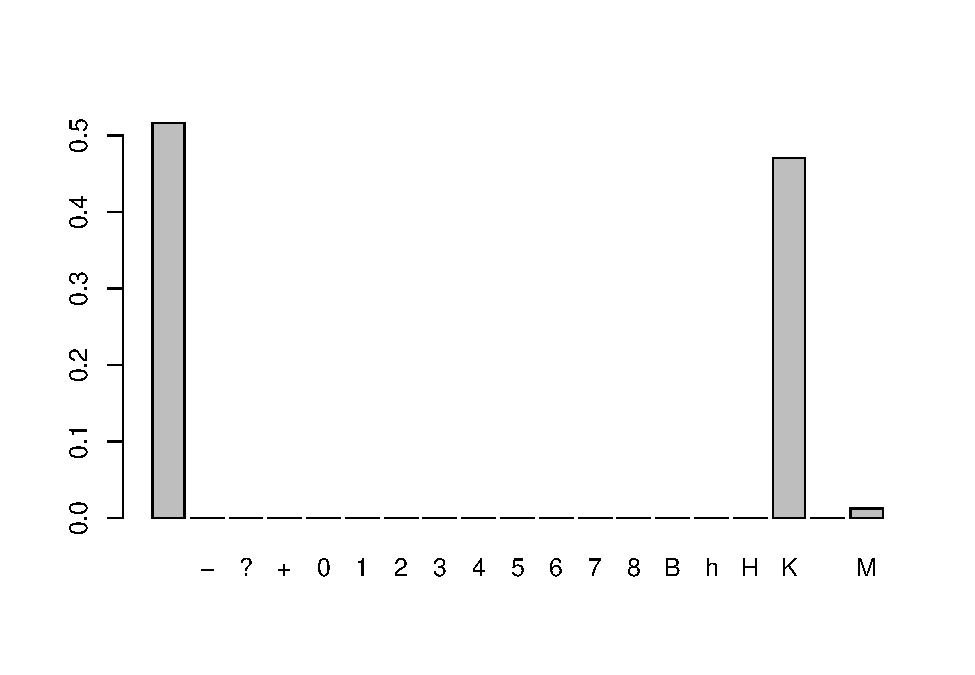
\includegraphics{RepData_PeerAssessment2_files/figure-latex/checking scales of damage-1.pdf}

\begin{Shaded}
\begin{Highlighting}[]
\FunctionTok{barplot}\NormalTok{(}\FunctionTok{prop.table}\NormalTok{(}\FunctionTok{table}\NormalTok{(Storm\_Data}\SpecialCharTok{$}\NormalTok{CROPDMGEXP)))}
\end{Highlighting}
\end{Shaded}

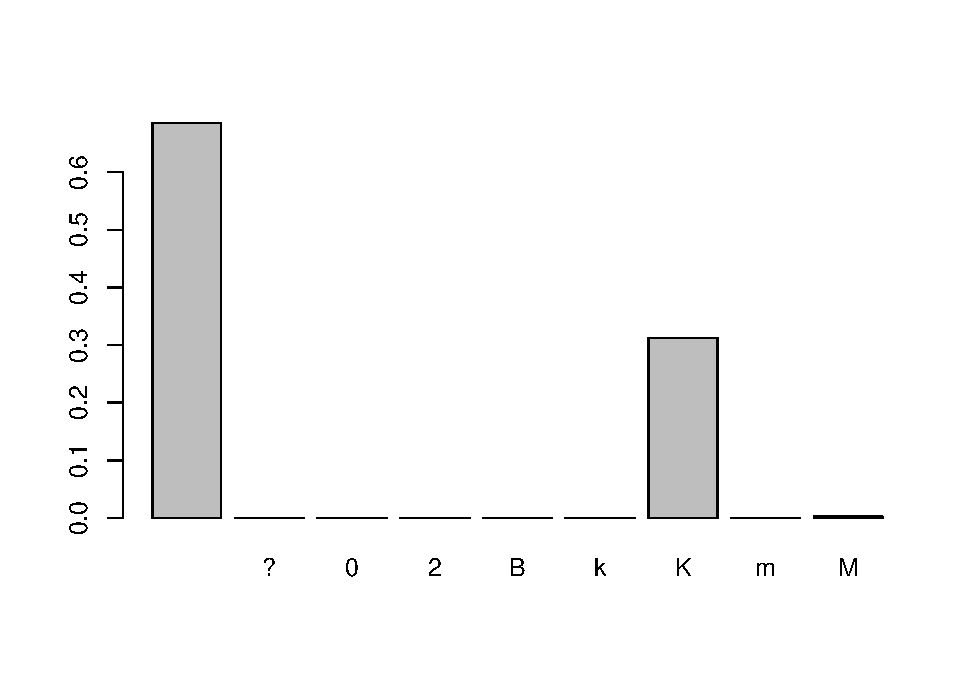
\includegraphics{RepData_PeerAssessment2_files/figure-latex/checking scales of damage-2.pdf}

Therefore, given the variety of multipliers, the following code chunk
will transform and present the damages as plain numbers. AS A SIDE NOTE,
initially, a loop line of code with i = {[}1 : N° of observations{]} was
formulated. However, it takes too long to compute the replacement with
it, and as such, Eric Brener's\footnote{\href{https://rpubs.com/EricTheBren/RepoResearchProj2}{Reproducible
  Research Peer-graded Assignment: Course Project 2} presents a very
  simple code chunk to replace the factor denominators.} work proved to
be a simpler, more streamlined and elegant solution. However, the
advantage of the loop method presented as inactive code is that instead
of replacing the denominators, it immediately would replace the
``factorized'' values for their actual values, e.g 11K for 11.000.

\begin{Shaded}
\begin{Highlighting}[]
\NormalTok{Damage\_Data}\SpecialCharTok{$}\NormalTok{PROPDMGEXP }\OtherTok{\textless{}{-}} 
  \FunctionTok{ifelse}\NormalTok{ (Damage\_Data}\SpecialCharTok{$}\NormalTok{PROPDMGEXP }\SpecialCharTok{==} \StringTok{"K"}\NormalTok{, }\FunctionTok{as.numeric}\NormalTok{(}\FunctionTok{format}\NormalTok{(}\DecValTok{1000}\NormalTok{, }\AttributeTok{scientific =} \ConstantTok{FALSE}\NormalTok{)),}
    \FunctionTok{ifelse}\NormalTok{ (Damage\_Data}\SpecialCharTok{$}\NormalTok{PROPDMGEXP }\SpecialCharTok{==} \StringTok{"M"}\NormalTok{, }\FunctionTok{as.numeric}\NormalTok{(}\FunctionTok{format}\NormalTok{(}\DecValTok{1000000}\NormalTok{, }\AttributeTok{scientific =} \ConstantTok{FALSE}\NormalTok{)),}
      \FunctionTok{ifelse}\NormalTok{ (Damage\_Data}\SpecialCharTok{$}\NormalTok{PROPDMGEXP }\SpecialCharTok{==} \StringTok{"m"}\NormalTok{, }\FunctionTok{as.numeric}\NormalTok{(}\FunctionTok{format}\NormalTok{(}\DecValTok{1000000}\NormalTok{, }\AttributeTok{scientific =} \ConstantTok{FALSE}\NormalTok{)),}
        \FunctionTok{ifelse}\NormalTok{ (Damage\_Data}\SpecialCharTok{$}\NormalTok{PROPDMGEXP }\SpecialCharTok{==} \StringTok{"B"}\NormalTok{, }\FunctionTok{as.numeric}\NormalTok{(}\FunctionTok{format}\NormalTok{(}\DecValTok{1000000000}\NormalTok{, }\AttributeTok{scientific =} \ConstantTok{FALSE}\NormalTok{)),}
          \FunctionTok{ifelse}\NormalTok{(Damage\_Data}\SpecialCharTok{$}\NormalTok{PROPDMGEXP }\SpecialCharTok{==} \StringTok{"H"}\NormalTok{, }\FunctionTok{as.numeric}\NormalTok{(}\FunctionTok{format}\NormalTok{(}\DecValTok{100}\NormalTok{, }\AttributeTok{scientific =} \ConstantTok{FALSE}\NormalTok{)),}
            \FunctionTok{ifelse}\NormalTok{(Damage\_Data}\SpecialCharTok{$}\NormalTok{PROPDMGEXP }\SpecialCharTok{==} \StringTok{"h"}\NormalTok{, }\FunctionTok{as.numeric}\NormalTok{(}\FunctionTok{format}\NormalTok{(}\DecValTok{100}\NormalTok{, }\AttributeTok{scientific =} \ConstantTok{FALSE}\NormalTok{)),}
              \FunctionTok{ifelse}\NormalTok{(Damage\_Data}\SpecialCharTok{$}\NormalTok{PROPDMGEXP }\SpecialCharTok{==} \StringTok{"1"}\NormalTok{, }\FunctionTok{as.numeric}\NormalTok{(}\FunctionTok{format}\NormalTok{(}\DecValTok{10}\NormalTok{, }\AttributeTok{scientific =} \ConstantTok{FALSE}\NormalTok{)),}
                \FunctionTok{ifelse}\NormalTok{(Damage\_Data}\SpecialCharTok{$}\NormalTok{PROPDMGEXP }\SpecialCharTok{==} \StringTok{"2"}\NormalTok{, }\FunctionTok{as.numeric}\NormalTok{(}\FunctionTok{format}\NormalTok{(}\DecValTok{100}\NormalTok{, }\AttributeTok{scientific =} \ConstantTok{FALSE}\NormalTok{)),}
                  \FunctionTok{ifelse}\NormalTok{(Damage\_Data}\SpecialCharTok{$}\NormalTok{PROPDMGEXP }\SpecialCharTok{==} \StringTok{"3"}\NormalTok{, }\FunctionTok{as.numeric}\NormalTok{(}\FunctionTok{format}\NormalTok{(}\DecValTok{1000}\NormalTok{, }\AttributeTok{scientific =} \ConstantTok{FALSE}\NormalTok{)),}
                    \FunctionTok{ifelse}\NormalTok{(Damage\_Data}\SpecialCharTok{$}\NormalTok{PROPDMGEXP }\SpecialCharTok{==} \StringTok{"4"}\NormalTok{, }\FunctionTok{as.numeric}\NormalTok{(}\FunctionTok{format}\NormalTok{(}\DecValTok{10000}\NormalTok{, }\AttributeTok{scientific =} \ConstantTok{FALSE}\NormalTok{)),}
                      \FunctionTok{ifelse}\NormalTok{(Damage\_Data}\SpecialCharTok{$}\NormalTok{PROPDMGEXP }\SpecialCharTok{==} \StringTok{"5"}\NormalTok{, }\FunctionTok{as.numeric}\NormalTok{(}\FunctionTok{format}\NormalTok{(}\DecValTok{100000}\NormalTok{, }\AttributeTok{scientific =} \ConstantTok{FALSE}\NormalTok{)),}
                        \FunctionTok{ifelse}\NormalTok{(Damage\_Data}\SpecialCharTok{$}\NormalTok{PROPDMGEXP }\SpecialCharTok{==} \StringTok{"6"}\NormalTok{, }\FunctionTok{as.numeric}\NormalTok{(}\FunctionTok{format}\NormalTok{(}\DecValTok{1000000}\NormalTok{, }\AttributeTok{scientific =} \ConstantTok{FALSE}\NormalTok{)),}
                          \FunctionTok{ifelse}\NormalTok{(Damage\_Data}\SpecialCharTok{$}\NormalTok{PROPDMGEXP }\SpecialCharTok{==} \StringTok{"7"}\NormalTok{, }\FunctionTok{as.numeric}\NormalTok{(}\FunctionTok{format}\NormalTok{(}\DecValTok{10000000}\NormalTok{, }\AttributeTok{scientific =} \ConstantTok{FALSE}\NormalTok{)),}
                            \FunctionTok{ifelse}\NormalTok{(Damage\_Data}\SpecialCharTok{$}\NormalTok{PROPDMGEXP }\SpecialCharTok{==} \StringTok{"8"}\NormalTok{, }\FunctionTok{as.numeric}\NormalTok{(}\FunctionTok{format}\NormalTok{(}\DecValTok{100000000}\NormalTok{, }\AttributeTok{scientific =} \ConstantTok{FALSE}\NormalTok{)),}
                            \FunctionTok{as.numeric}\NormalTok{(}\DecValTok{1}\NormalTok{)))))))))))))))}

\NormalTok{Damage\_Data}\SpecialCharTok{$}\NormalTok{PROPDMG }\OtherTok{\textless{}{-}}\NormalTok{ (Damage\_Data}\SpecialCharTok{$}\NormalTok{PROPDMG }\SpecialCharTok{*}\NormalTok{ Damage\_Data}\SpecialCharTok{$}\NormalTok{PROPDMGEXP)}

\NormalTok{Damage\_Data}\SpecialCharTok{$}\NormalTok{CROPDMGEXP }\OtherTok{\textless{}{-}}
  \FunctionTok{ifelse}\NormalTok{ (Damage\_Data}\SpecialCharTok{$}\NormalTok{CROPDMGEXP }\SpecialCharTok{==} \StringTok{"K"}\NormalTok{, }\FunctionTok{as.numeric}\NormalTok{(}\FunctionTok{format}\NormalTok{(}\DecValTok{1000}\NormalTok{, }\AttributeTok{scientific =} \ConstantTok{FALSE}\NormalTok{)),}
    \FunctionTok{ifelse}\NormalTok{ (Damage\_Data}\SpecialCharTok{$}\NormalTok{CROPDMGEXP }\SpecialCharTok{==} \StringTok{"k"}\NormalTok{, }\FunctionTok{as.numeric}\NormalTok{(}\FunctionTok{format}\NormalTok{(}\DecValTok{1000}\NormalTok{, }\AttributeTok{scientific =} \ConstantTok{FALSE}\NormalTok{)),}
      \FunctionTok{ifelse}\NormalTok{ (Damage\_Data}\SpecialCharTok{$}\NormalTok{CROPDMGEXP }\SpecialCharTok{==} \StringTok{"M"}\NormalTok{, }\FunctionTok{as.numeric}\NormalTok{(}\FunctionTok{format}\NormalTok{(}\DecValTok{1000000}\NormalTok{, }\AttributeTok{scientific =} \ConstantTok{FALSE}\NormalTok{)),}
        \FunctionTok{ifelse}\NormalTok{(Damage\_Data}\SpecialCharTok{$}\NormalTok{CROPDMGEXP }\SpecialCharTok{==} \StringTok{"m"}\NormalTok{, }\FunctionTok{as.numeric}\NormalTok{(}\FunctionTok{format}\NormalTok{(}\DecValTok{1000000}\NormalTok{, }\AttributeTok{scientific =} \ConstantTok{FALSE}\NormalTok{)),}
          \FunctionTok{ifelse}\NormalTok{(Damage\_Data}\SpecialCharTok{$}\NormalTok{CROPDMGEXP }\SpecialCharTok{==} \StringTok{"B"}\NormalTok{, }\FunctionTok{as.numeric}\NormalTok{(}\FunctionTok{format}\NormalTok{(}\DecValTok{1000000000}\NormalTok{, }\AttributeTok{scientific =} \ConstantTok{FALSE}\NormalTok{)),}
            \FunctionTok{ifelse}\NormalTok{(Damage\_Data}\SpecialCharTok{$}\NormalTok{CROPDMGEXP }\SpecialCharTok{==} \StringTok{"2"}\NormalTok{, }\FunctionTok{as.numeric}\NormalTok{(}\FunctionTok{format}\NormalTok{(}\DecValTok{100}\NormalTok{, }\AttributeTok{scientific =} \ConstantTok{FALSE}\NormalTok{)),}
              \FunctionTok{as.numeric}\NormalTok{(}\DecValTok{1}\NormalTok{)))))))}

\NormalTok{Damage\_Data}\SpecialCharTok{$}\NormalTok{CROPDMG }\OtherTok{\textless{}{-}}\NormalTok{ (Damage\_Data}\SpecialCharTok{$}\NormalTok{CROPDMG }\SpecialCharTok{*}\NormalTok{ Damage\_Data}\SpecialCharTok{$}\NormalTok{CROPDMGEXP)}

\NormalTok{Damage\_Data }\OtherTok{\textless{}{-}} \FunctionTok{subset}\NormalTok{(Damage\_Data, }\AttributeTok{select =} \SpecialCharTok{{-}}\NormalTok{CROPDMGEXP)}
\NormalTok{Damage\_Data }\OtherTok{\textless{}{-}} \FunctionTok{subset}\NormalTok{(Damage\_Data, }\AttributeTok{select =} \SpecialCharTok{{-}}\NormalTok{PROPDMGEXP)}

\CommentTok{\#for (i in 1:length(Damage\_Data$BGN\_DATE)) \{}
\CommentTok{\#  if(Damage\_Data$PROPDMGEXP[i] == "K") \{}
\CommentTok{\#    Damage\_Data$PROPDMG[i] \textless{}{-} Damage\_Data$PROPDMG[i] * 1000}
\CommentTok{\#    \}}
\CommentTok{\#  else if(Damage\_Data$PROPDMGEXP[i] == "M") \{}
\CommentTok{\#    Damage\_Data$PROPDMG[i] \textless{}{-} Damage\_Data$PROPDMG[i] * 1000000}
\CommentTok{\#    \}}
\CommentTok{\#  else if(Damage\_Data$PROPDMGEXP[i] == "h") \{}
\CommentTok{\#    Damage\_Data$PROPDMG[i] \textless{}{-} Damage\_Data$PROPDMG[i] * 100}
\CommentTok{\#    \}}
\CommentTok{\#  else if(Damage\_Data$PROPDMGEXP[i] == "B") \{}
\CommentTok{\#    Damage\_Data$PROPDMG[i] \textless{}{-} Damage\_Data$PROPDMG[i] * 1000000000}
\CommentTok{\#    \}}
\CommentTok{\#  else \{}
\CommentTok{\#    Damage\_Data$PROPDMG[i] \textless{}{-} Damage\_Data$PROPDMG[i] * 1}
\CommentTok{\#    \}}
\CommentTok{\#\}}

\CommentTok{\#for (j in 1:length(Damage\_Data$BGN\_DATE)) \{}
\CommentTok{\#  if(Damage\_Data$CROPDMGEXP[j] == "K") \{}
\CommentTok{\#    Damage\_Data$CROPDMG[j] \textless{}{-} Damage\_Data$CROPDMG[j] * 1000}
\CommentTok{\#    \}}
\CommentTok{\#  else if(Damage\_Data$CROPDMGEXP[j] == "k") \{}
\CommentTok{\#    Damage\_Data$CROPDMG[j] \textless{}{-} Damage\_Data$CROPDMG[j] * 1000}
\CommentTok{\#    \}}
\CommentTok{\#  else if(Damage\_Data$CROPDMGEXP[j] == "M") \{}
\CommentTok{\#    Damage\_Data$CROPDMG[j] \textless{}{-} Damage\_Data$CROPDMG[j] * 1000000}
\CommentTok{\#    \}}
\CommentTok{\#  else if(Damage\_Data$CROPDMGEXP[j] == "m") \{}
\CommentTok{\#    Damage\_Data$CROPDMG[j] \textless{}{-} Damage\_Data$CROPDMG[j] * 1000000}
\CommentTok{\#    \}}
\CommentTok{\#  else if(Damage\_Data$CROPDMGEXP[j] == "B") \{}
\CommentTok{\#    Damage\_Data$CROPDMG[j] \textless{}{-} Damage\_Data$CROPDMG[j] * 1000000000}
\CommentTok{\#    \}}
\CommentTok{\#  else \{}
\CommentTok{\#    Damage\_Data$CROPDMG[j] \textless{}{-} Damage\_Data$CROPDMG[j] * 1}
\CommentTok{\#    \}}
\CommentTok{\#\}}
\end{Highlighting}
\end{Shaded}

Now that the data has been simplified, it must be aggregated. As such,
the following chunk sums the injuries, fatalities, property damage
values, and crop damage values, subtotaling by year and event type.
HOWEVER, given that the objective is to get a comprehensive analysis by
year AND by type of event, it should be convenient to count the types of
events, which, according to the following code, amount to:

\begin{Shaded}
\begin{Highlighting}[]
\FunctionTok{length}\NormalTok{(}\FunctionTok{unique}\NormalTok{(Damage\_Data}\SpecialCharTok{$}\NormalTok{EVTYPE))}
\end{Highlighting}
\end{Shaded}

\begin{verbatim}
## [1] 985
\end{verbatim}

Which would mean the same number of plotlines, or even subplots would be
generated. Therefore, it is a sensible move to compile the events in
more generalized categories, which can be done by means of regular
expressions, as done by Joel Tworek\footnote{\href{https://rpubs.com/JoelTK/205449}{JoelTK's
  Reproducible Research: Peer Assignment 2} provides the means to
  summarize almost a thousand types of events into 14 categories.}.

\begin{Shaded}
\begin{Highlighting}[]
\NormalTok{Damage\_Data}\SpecialCharTok{$}\NormalTok{Event\_Category }\OtherTok{\textless{}{-}} \FunctionTok{ifelse}\NormalTok{(}\FunctionTok{grepl}\NormalTok{(}\StringTok{"LIGHTNING|LIGNTNING"}\NormalTok{, Damage\_Data}\SpecialCharTok{$}\NormalTok{EVTYPE), }\StringTok{"LIGHTNING"}\NormalTok{, }
    \FunctionTok{ifelse}\NormalTok{(}\FunctionTok{grepl}\NormalTok{(}\StringTok{"RAIN|FLOOD|WET|FLD"}\NormalTok{, Damage\_Data}\SpecialCharTok{$}\NormalTok{EVTYPE), }\StringTok{"RAIN {-} WATER"}\NormalTok{,}
      \FunctionTok{ifelse}\NormalTok{(}\FunctionTok{grepl}\NormalTok{(}\StringTok{"HAIL|SNOW|WINTER|WINTRY|BLIZZARD|SLEET|COLD|ICE|FREEZE|AVALANCHE|ICY"}\NormalTok{, Damage\_Data}\SpecialCharTok{$}\NormalTok{EVTYPE), }\StringTok{"WINTER {-} FREEZING PRECIPITATION"}\NormalTok{,}
       \FunctionTok{ifelse}\NormalTok{(}\FunctionTok{grepl}\NormalTok{(}\StringTok{"TORNADO|FUNNEL|WIND|HURRICANE"}\NormalTok{, Damage\_Data}\SpecialCharTok{$}\NormalTok{EVTYPE), }\StringTok{"HURRICANE {-} TORNADO {-} HIGH WINDS"}\NormalTok{,}
        \FunctionTok{ifelse}\NormalTok{(}\FunctionTok{grepl}\NormalTok{(}\StringTok{"STORM|THUNDER|TSTM|TROPICAL +STORM"}\NormalTok{, Damage\_Data}\SpecialCharTok{$}\NormalTok{EVTYPE), }\StringTok{"STORM"}\NormalTok{,}
          \FunctionTok{ifelse}\NormalTok{(}\FunctionTok{grepl}\NormalTok{(}\StringTok{"FIRE"}\NormalTok{, Damage\_Data}\SpecialCharTok{$}\NormalTok{EVTYPE), }\StringTok{"FIRE"}\NormalTok{,}
           \FunctionTok{ifelse}\NormalTok{(}\FunctionTok{grepl}\NormalTok{(}\StringTok{"FOG|VISIBILITY|DARK|DUST"}\NormalTok{, Damage\_Data}\SpecialCharTok{$}\NormalTok{EVTYPE), }\StringTok{"REDUCED VISIBILITY"}\NormalTok{,}
            \FunctionTok{ifelse}\NormalTok{(}\FunctionTok{grepl}\NormalTok{(}\StringTok{"WAVE|SURF|SURGE|TIDE|TSUNAMI|CURRENT|SWELL"}\NormalTok{, Damage\_Data}\SpecialCharTok{$}\NormalTok{EVTYPE), }\StringTok{"MARITIME EVENTS"}\NormalTok{,}
             \FunctionTok{ifelse}\NormalTok{(}\FunctionTok{grepl}\NormalTok{(}\StringTok{"HEAT|HIGH +TEMP|RECORD +TEMP|WARM|DRY"}\NormalTok{, Damage\_Data}\SpecialCharTok{$}\NormalTok{EVTYPE), }\StringTok{"HIGH TEMPERATURES"}\NormalTok{,}
              \FunctionTok{ifelse}\NormalTok{(}\FunctionTok{grepl}\NormalTok{(}\StringTok{"VOLCAN"}\NormalTok{, Damage\_Data}\SpecialCharTok{$}\NormalTok{EVTYPE), }\StringTok{"VOLCANO"}\NormalTok{,}
               \FunctionTok{ifelse}\NormalTok{(}\FunctionTok{grepl}\NormalTok{(}\StringTok{"DROUGHT"}\NormalTok{, Damage\_Data}\SpecialCharTok{$}\NormalTok{EVTYPE), }\StringTok{"DROUGHT"}\NormalTok{,}
               \StringTok{"OTHER"}\NormalTok{)))))))))))}

\NormalTok{Casualties\_Data}\SpecialCharTok{$}\NormalTok{Event\_Category }\OtherTok{\textless{}{-}} \FunctionTok{ifelse}\NormalTok{(}\FunctionTok{grepl}\NormalTok{(}\StringTok{"LIGHTNING|LIGNTNING"}\NormalTok{, Casualties\_Data}\SpecialCharTok{$}\NormalTok{EVTYPE), }\StringTok{"LIGHTNING"}\NormalTok{, }
    \FunctionTok{ifelse}\NormalTok{(}\FunctionTok{grepl}\NormalTok{(}\StringTok{"RAIN|FLOOD|WET|FLD"}\NormalTok{, Casualties\_Data}\SpecialCharTok{$}\NormalTok{EVTYPE), }\StringTok{"RAIN {-} WATER"}\NormalTok{,}
      \FunctionTok{ifelse}\NormalTok{(}\FunctionTok{grepl}\NormalTok{(}\StringTok{"HAIL|SNOW|WINTER|WINTRY|BLIZZARD|SLEET|COLD|ICE|FREEZE|AVALANCHE|ICY"}\NormalTok{, Casualties\_Data}\SpecialCharTok{$}\NormalTok{EVTYPE), }\StringTok{"WINTER {-} FREEZING PRECIPITATION"}\NormalTok{,}
       \FunctionTok{ifelse}\NormalTok{(}\FunctionTok{grepl}\NormalTok{(}\StringTok{"TORNADO|FUNNEL|WIND|HURRICANE"}\NormalTok{, Casualties\_Data}\SpecialCharTok{$}\NormalTok{EVTYPE), }\StringTok{"HURRICANE {-} TORNADO {-} HIGH WINDS"}\NormalTok{,}
        \FunctionTok{ifelse}\NormalTok{(}\FunctionTok{grepl}\NormalTok{(}\StringTok{"STORM|THUNDER|TSTM|TROPICAL +STORM"}\NormalTok{, Casualties\_Data}\SpecialCharTok{$}\NormalTok{EVTYPE), }\StringTok{"STORM"}\NormalTok{,}
          \FunctionTok{ifelse}\NormalTok{(}\FunctionTok{grepl}\NormalTok{(}\StringTok{"FIRE"}\NormalTok{, Casualties\_Data}\SpecialCharTok{$}\NormalTok{EVTYPE), }\StringTok{"FIRE"}\NormalTok{,}
           \FunctionTok{ifelse}\NormalTok{(}\FunctionTok{grepl}\NormalTok{(}\StringTok{"FOG|VISIBILITY|DARK|DUST"}\NormalTok{, Casualties\_Data}\SpecialCharTok{$}\NormalTok{EVTYPE), }\StringTok{"REDUCED VISIBILITY"}\NormalTok{,}
            \FunctionTok{ifelse}\NormalTok{(}\FunctionTok{grepl}\NormalTok{(}\StringTok{"WAVE|SURF|SURGE|TIDE|TSUNAMI|CURRENT|SWELL"}\NormalTok{, Casualties\_Data}\SpecialCharTok{$}\NormalTok{EVTYPE), }\StringTok{"MARITIME EVENTS"}\NormalTok{,}
             \FunctionTok{ifelse}\NormalTok{(}\FunctionTok{grepl}\NormalTok{(}\StringTok{"HEAT|HIGH +TEMP|RECORD +TEMP|WARM|DRY"}\NormalTok{, Casualties\_Data}\SpecialCharTok{$}\NormalTok{EVTYPE), }\StringTok{"HIGH TEMPERATURES"}\NormalTok{,}
              \FunctionTok{ifelse}\NormalTok{(}\FunctionTok{grepl}\NormalTok{(}\StringTok{"VOLCAN"}\NormalTok{, Casualties\_Data}\SpecialCharTok{$}\NormalTok{EVTYPE), }\StringTok{"VOLCANO"}\NormalTok{,}
               \FunctionTok{ifelse}\NormalTok{(}\FunctionTok{grepl}\NormalTok{(}\StringTok{"DROUGHT"}\NormalTok{, Casualties\_Data}\SpecialCharTok{$}\NormalTok{EVTYPE), }\StringTok{"DROUGHT"}\NormalTok{,}
               \StringTok{"OTHER"}\NormalTok{)))))))))))}

\CommentTok{\#Again, in order to preserve the original dataframe, the code is used redundantly for both sub{-}frames.}

\FunctionTok{paste}\NormalTok{(}\StringTok{"The"}\NormalTok{, }\FunctionTok{length}\NormalTok{(}\FunctionTok{unique}\NormalTok{(Damage\_Data}\SpecialCharTok{$}\NormalTok{EVTYPE)), }\StringTok{"event types are compiled into"}\NormalTok{, }\FunctionTok{length}\NormalTok{(}\FunctionTok{unique}\NormalTok{(Damage\_Data}\SpecialCharTok{$}\NormalTok{Event\_Category)), }\StringTok{"categories, which are:"}\NormalTok{)}
\end{Highlighting}
\end{Shaded}

\begin{verbatim}
## [1] "The 985 event types are compiled into 12 categories, which are:"
\end{verbatim}

\begin{Shaded}
\begin{Highlighting}[]
\FunctionTok{unique}\NormalTok{(Damage\_Data}\SpecialCharTok{$}\NormalTok{Event\_Category)}
\end{Highlighting}
\end{Shaded}

\begin{verbatim}
##  [1] "HURRICANE - TORNADO - HIGH WINDS" "WINTER - FREEZING PRECIPITATION" 
##  [3] "RAIN - WATER"                     "LIGHTNING"                       
##  [5] "REDUCED VISIBILITY"               "MARITIME EVENTS"                 
##  [7] "STORM"                            "HIGH TEMPERATURES"               
##  [9] "OTHER"                            "FIRE"                            
## [11] "DROUGHT"                          "VOLCANO"
\end{verbatim}

So, after (1) obtaining the data, (2) analyzing it and getting a grasp
regarding the way it was framed, (3) transforming it so that it can be
worked with, and (4) summarizing the numerous types of weather events
into just a dozen, the data can be finally (5) aggregated by the kind of
weather events and by time.

\begin{Shaded}
\begin{Highlighting}[]
\NormalTok{Damage\_aggregation }\OtherTok{\textless{}{-}} \FunctionTok{aggregate}\NormalTok{(}\FunctionTok{list}\NormalTok{(}\AttributeTok{Property\_Damage =}\NormalTok{ Damage\_Data}\SpecialCharTok{$}\NormalTok{PROPDMG, }\AttributeTok{Crops\_Damage =}\NormalTok{ Damage\_Data}\SpecialCharTok{$}\NormalTok{CROPDMG), }\AttributeTok{by =} \FunctionTok{list}\NormalTok{(}\AttributeTok{Event =}\NormalTok{ Damage\_Data}\SpecialCharTok{$}\NormalTok{Event\_Category, }\AttributeTok{year =}\NormalTok{ Damage\_Data}\SpecialCharTok{$}\NormalTok{BGN\_DATE), }\AttributeTok{na.rm =} \ConstantTok{TRUE}\NormalTok{, }\AttributeTok{FUN =}\NormalTok{ sum)}

\NormalTok{Damage\_total }\OtherTok{\textless{}{-}} \FunctionTok{aggregate}\NormalTok{(}\FunctionTok{list}\NormalTok{(}\AttributeTok{Property\_Damage =}\NormalTok{ Damage\_Data}\SpecialCharTok{$}\NormalTok{PROPDMG, }\AttributeTok{Crops\_Damage =}\NormalTok{ Damage\_Data}\SpecialCharTok{$}\NormalTok{CROPDMG), }\AttributeTok{by =} \FunctionTok{list}\NormalTok{(}\AttributeTok{Event =}\NormalTok{ Damage\_Data}\SpecialCharTok{$}\NormalTok{Event\_Category), }\AttributeTok{na.rm =} \ConstantTok{TRUE}\NormalTok{, }\AttributeTok{FUN =}\NormalTok{ sum)}

\NormalTok{Casualties\_aggregation }\OtherTok{\textless{}{-}} \FunctionTok{aggregate}\NormalTok{(}\FunctionTok{list}\NormalTok{(}\AttributeTok{Fatalities =}\NormalTok{ Casualties\_Data}\SpecialCharTok{$}\NormalTok{FATALITIES, }\AttributeTok{Injuries =}\NormalTok{ Casualties\_Data}\SpecialCharTok{$}\NormalTok{INJURIES), }\AttributeTok{by =} \FunctionTok{list}\NormalTok{(}\AttributeTok{Event =}\NormalTok{ Casualties\_Data}\SpecialCharTok{$}\NormalTok{Event\_Category, }\AttributeTok{year =}\NormalTok{ Casualties\_Data}\SpecialCharTok{$}\NormalTok{BGN\_DATE), }\AttributeTok{na.rm =} \ConstantTok{TRUE}\NormalTok{, }\AttributeTok{FUN =}\NormalTok{ sum)}

\NormalTok{Casualties\_total }\OtherTok{\textless{}{-}} \FunctionTok{aggregate}\NormalTok{(}\FunctionTok{list}\NormalTok{(}\AttributeTok{Fatalities =}\NormalTok{ Casualties\_Data}\SpecialCharTok{$}\NormalTok{FATALITIES, }\AttributeTok{Injuries =}\NormalTok{ Casualties\_Data}\SpecialCharTok{$}\NormalTok{INJURIES), }\AttributeTok{by =} \FunctionTok{list}\NormalTok{(}\AttributeTok{Event =}\NormalTok{ Casualties\_Data}\SpecialCharTok{$}\NormalTok{Event\_Category), }\AttributeTok{na.rm =} \ConstantTok{TRUE}\NormalTok{, }\AttributeTok{FUN =}\NormalTok{ sum)}
\end{Highlighting}
\end{Shaded}

So, the data can finally be (6) analyzed to determine which weather
events are more damaging to property and which are more lethal

\hypertarget{results}{%
\subsection{Results}\label{results}}

\hypertarget{its-relevant-to-mention-that-because-of-an-almost-exponential-difference-in-the-values-between-the-events-each-plot-has-its-own-scale-for-the-y-axis-so-it-should-be-taken-in-consideration.-when-looking-at-each-plot.}{%
\paragraph{It's relevant to mention that, because of an almost
exponential difference in the values between the events, each plot has
its own scale for the y axis, so it should be taken in consideration.
when looking at each
plot.}\label{its-relevant-to-mention-that-because-of-an-almost-exponential-difference-in-the-values-between-the-events-each-plot-has-its-own-scale-for-the-y-axis-so-it-should-be-taken-in-consideration.-when-looking-at-each-plot.}}

\begin{Shaded}
\begin{Highlighting}[]
\FunctionTok{library}\NormalTok{(ggplot2)}
\FunctionTok{options}\NormalTok{(}\AttributeTok{scipen=}\DecValTok{999}\NormalTok{)}

\NormalTok{propdmg }\OtherTok{\textless{}{-}} \FunctionTok{ggplot}\NormalTok{(Damage\_total, }\FunctionTok{aes}\NormalTok{(Event, Property\_Damage))}
\NormalTok{propdmg }\OtherTok{\textless{}{-}}\NormalTok{ propdmg }\SpecialCharTok{+} \FunctionTok{geom\_bar}\NormalTok{(}\AttributeTok{stat=}\StringTok{"identity"}\NormalTok{, }\AttributeTok{position =} \StringTok{"dodge"}\NormalTok{) }\SpecialCharTok{+} \FunctionTok{ggtitle}\NormalTok{(}\StringTok{"Property Damage vs Event Category"}\NormalTok{) }\SpecialCharTok{+} \FunctionTok{theme}\NormalTok{(}\AttributeTok{axis.text.x =} \FunctionTok{element\_text}\NormalTok{(}\AttributeTok{angle =} \DecValTok{90}\NormalTok{))}
\NormalTok{propdmg }\OtherTok{\textless{}{-}}\NormalTok{ propdmg }\SpecialCharTok{+} \FunctionTok{scale\_y\_continuous}\NormalTok{(}\AttributeTok{labels =}\NormalTok{ scales}\SpecialCharTok{::}\NormalTok{comma)}
\FunctionTok{print}\NormalTok{(propdmg)}
\end{Highlighting}
\end{Shaded}

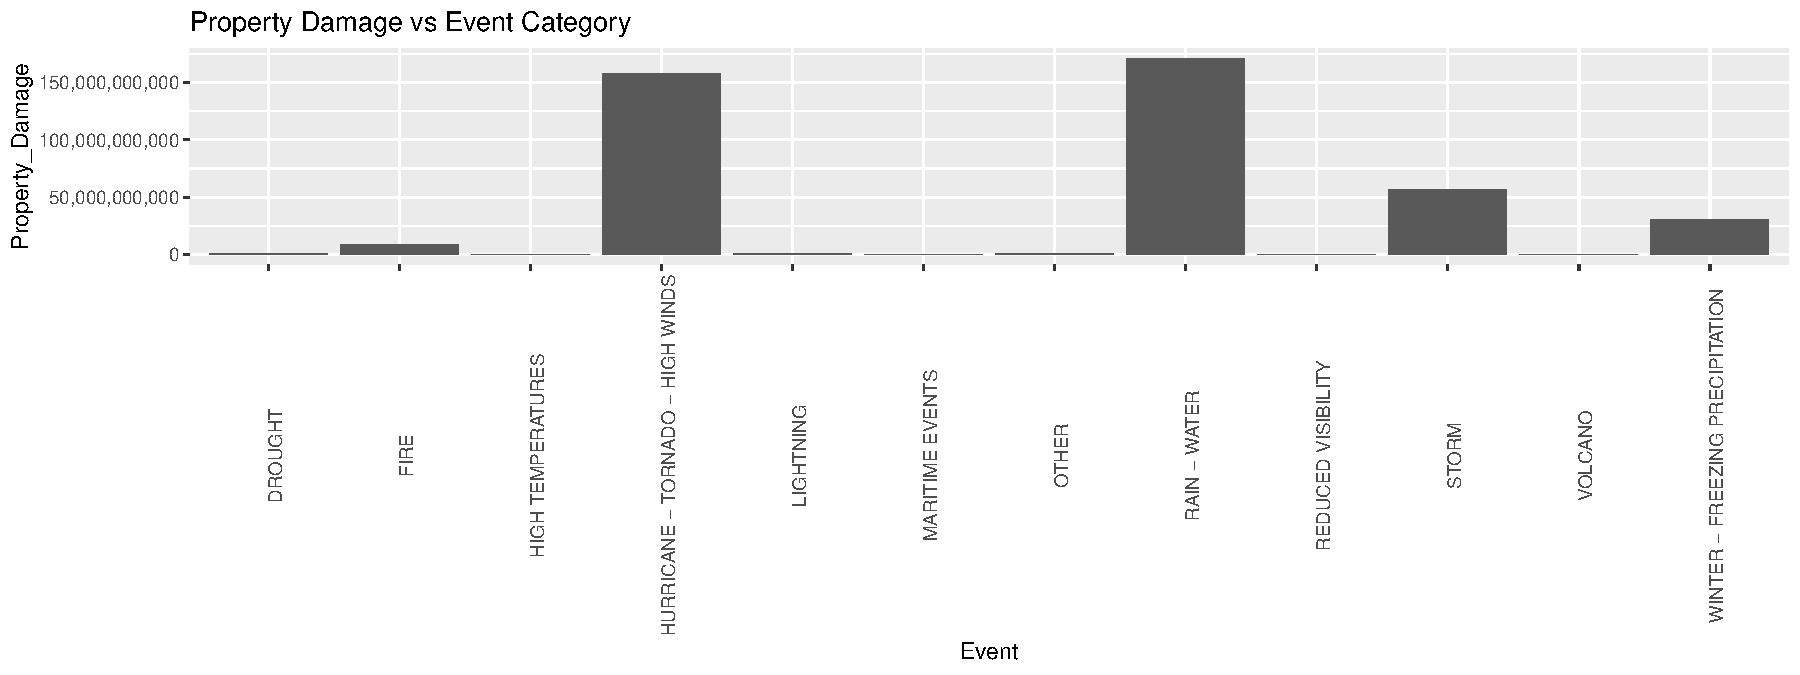
\includegraphics{RepData_PeerAssessment2_files/figure-latex/Property Results-1.pdf}

\begin{Shaded}
\begin{Highlighting}[]
\NormalTok{propdmg\_vs\_year}\OtherTok{\textless{}{-}} \FunctionTok{ggplot}\NormalTok{(Damage\_aggregation, }\FunctionTok{aes}\NormalTok{(year, Property\_Damage, }\AttributeTok{fill =}\NormalTok{ Event))}
\NormalTok{propdmg\_vs\_year }\OtherTok{\textless{}{-}}\NormalTok{ propdmg\_vs\_year }\SpecialCharTok{+} \FunctionTok{geom\_bar}\NormalTok{(}\AttributeTok{stat=}\StringTok{"identity"}\NormalTok{) }\SpecialCharTok{+} \FunctionTok{ggtitle}\NormalTok{(}\StringTok{"Yearly Property Damage by Event"}\NormalTok{) }\SpecialCharTok{+} \FunctionTok{facet\_wrap}\NormalTok{(.}\SpecialCharTok{\textasciitilde{}}\NormalTok{Event, }\AttributeTok{scales =} \StringTok{"free\_y"}\NormalTok{) }\SpecialCharTok{+} \FunctionTok{theme}\NormalTok{(}\AttributeTok{axis.text.x =} \FunctionTok{element\_text}\NormalTok{(}\AttributeTok{angle =} \DecValTok{90}\NormalTok{))}
\NormalTok{propdmg\_vs\_year }\OtherTok{\textless{}{-}}\NormalTok{ propdmg\_vs\_year }\SpecialCharTok{+} \FunctionTok{scale\_y\_continuous}\NormalTok{(}\AttributeTok{labels =}\NormalTok{ scales}\SpecialCharTok{::}\NormalTok{comma) }\SpecialCharTok{+} \FunctionTok{coord\_cartesian}\NormalTok{(}\AttributeTok{xlim =} \FunctionTok{c}\NormalTok{(}\DecValTok{1970}\NormalTok{, }\DecValTok{2011}\NormalTok{))}
\FunctionTok{print}\NormalTok{(propdmg\_vs\_year)}
\end{Highlighting}
\end{Shaded}

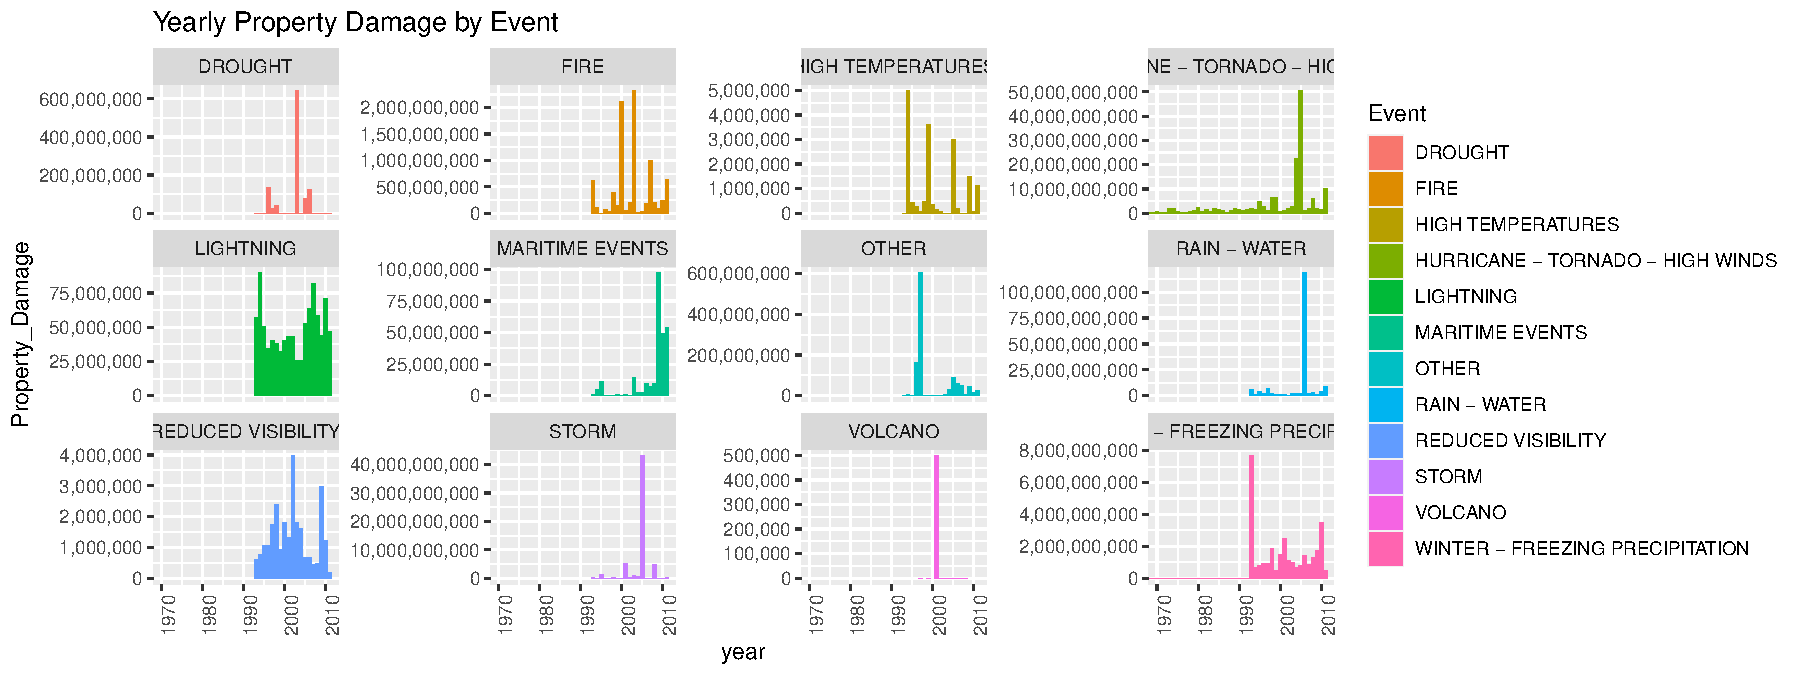
\includegraphics{RepData_PeerAssessment2_files/figure-latex/Property Results-2.pdf}

So, it is clear that, accumulated over the years, Rain, Floods and other
Water related weather events have caused the most property damage,
followed very closely by Hurricanes, Tornadoes and High Winds.

Nevertheless, the damage done by tornadoes clearly has been measured
SINCE a lot earlier than other events, and, although the lack of
observations for the RAIN-WATER category could be attributed to the
recent HIGHLY VISIBLE effects of climate change, it's more likely that
it is a lack of data what gives high winds its 2° place.

\hypertarget{so-heavy-rains-and-floods-are-likely-to-be-the-most-damaging-weather-phenomena-towards-property-but-when-looked-from-a-a-continuity-point-of-if-view-if-in-fact-floods-and-heavy-rain-were-not-a-problem-prior-to-1990-perhaps-hurricanes-and-tornadoes-have-been-a-bigger-threat.}{%
\paragraph{So, Heavy Rains and Floods are likely to be the most damaging
weather phenomena towards property, but when looked from a a
``continuity'' point of if view, if in fact, floods and heavy rain were
not a problem prior to 1990, perhaps hurricanes and tornadoes have been
a bigger
threat.}\label{so-heavy-rains-and-floods-are-likely-to-be-the-most-damaging-weather-phenomena-towards-property-but-when-looked-from-a-a-continuity-point-of-if-view-if-in-fact-floods-and-heavy-rain-were-not-a-problem-prior-to-1990-perhaps-hurricanes-and-tornadoes-have-been-a-bigger-threat.}}

\begin{Shaded}
\begin{Highlighting}[]
\FunctionTok{library}\NormalTok{(ggplot2)}
\FunctionTok{options}\NormalTok{(}\AttributeTok{scipen=}\DecValTok{999}\NormalTok{)}

\NormalTok{cropdmg }\OtherTok{\textless{}{-}} \FunctionTok{ggplot}\NormalTok{(Damage\_total, }\FunctionTok{aes}\NormalTok{(Event, Crops\_Damage))}
\NormalTok{cropdmg }\OtherTok{\textless{}{-}}\NormalTok{ cropdmg }\SpecialCharTok{+} \FunctionTok{geom\_bar}\NormalTok{(}\AttributeTok{stat=}\StringTok{"identity"}\NormalTok{, }\AttributeTok{position =} \StringTok{"dodge"}\NormalTok{) }\SpecialCharTok{+} \FunctionTok{ggtitle}\NormalTok{(}\StringTok{"Crops Damage vs Event Category"}\NormalTok{) }\SpecialCharTok{+} \FunctionTok{theme}\NormalTok{(}\AttributeTok{axis.text.x =} \FunctionTok{element\_text}\NormalTok{(}\AttributeTok{angle =} \DecValTok{90}\NormalTok{))}
\NormalTok{cropdmg }\OtherTok{\textless{}{-}}\NormalTok{ cropdmg }\SpecialCharTok{+} \FunctionTok{scale\_y\_continuous}\NormalTok{(}\AttributeTok{labels =}\NormalTok{ scales}\SpecialCharTok{::}\NormalTok{comma)}
\FunctionTok{print}\NormalTok{(cropdmg)}
\end{Highlighting}
\end{Shaded}

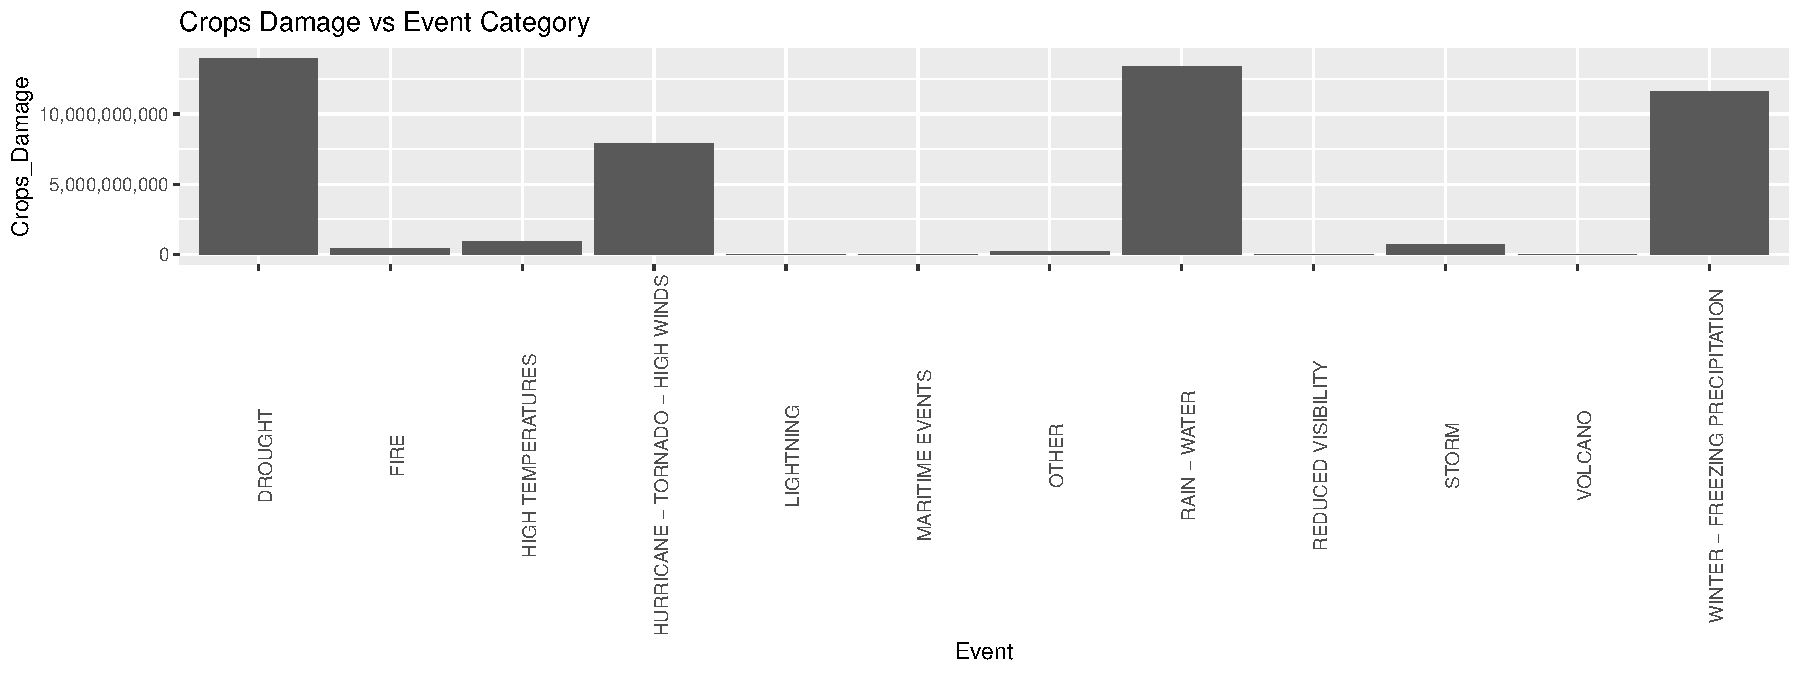
\includegraphics{RepData_PeerAssessment2_files/figure-latex/Crops Results-1.pdf}

\begin{Shaded}
\begin{Highlighting}[]
\NormalTok{cropdmg\_vs\_year}\OtherTok{\textless{}{-}} \FunctionTok{ggplot}\NormalTok{(Damage\_aggregation, }\FunctionTok{aes}\NormalTok{(year, Crops\_Damage, }\AttributeTok{fill =}\NormalTok{ Event))}
\NormalTok{cropdmg\_vs\_year }\OtherTok{\textless{}{-}}\NormalTok{ cropdmg\_vs\_year }\SpecialCharTok{+} \FunctionTok{geom\_bar}\NormalTok{(}\AttributeTok{stat=}\StringTok{"identity"}\NormalTok{, }\AttributeTok{position =} \StringTok{"dodge"}\NormalTok{) }\SpecialCharTok{+} \FunctionTok{ggtitle}\NormalTok{(}\StringTok{"Yearly Crops Damage by Event"}\NormalTok{)}\SpecialCharTok{+} \FunctionTok{facet\_wrap}\NormalTok{(.}\SpecialCharTok{\textasciitilde{}}\NormalTok{Event, }\AttributeTok{scales =} \StringTok{"free\_y"}\NormalTok{) }\SpecialCharTok{+} \FunctionTok{theme}\NormalTok{(}\AttributeTok{axis.text.x =} \FunctionTok{element\_text}\NormalTok{(}\AttributeTok{angle =} \DecValTok{90}\NormalTok{))}
\NormalTok{cropdmg\_vs\_year }\OtherTok{\textless{}{-}}\NormalTok{ cropdmg\_vs\_year  }\SpecialCharTok{+} \FunctionTok{scale\_y\_continuous}\NormalTok{(}\AttributeTok{labels =}\NormalTok{ scales}\SpecialCharTok{::}\NormalTok{comma) }\SpecialCharTok{+} \FunctionTok{coord\_cartesian}\NormalTok{(}\AttributeTok{xlim =} \FunctionTok{c}\NormalTok{(}\DecValTok{1990}\NormalTok{, }\DecValTok{2011}\NormalTok{))}
\FunctionTok{print}\NormalTok{(cropdmg\_vs\_year)}
\end{Highlighting}
\end{Shaded}

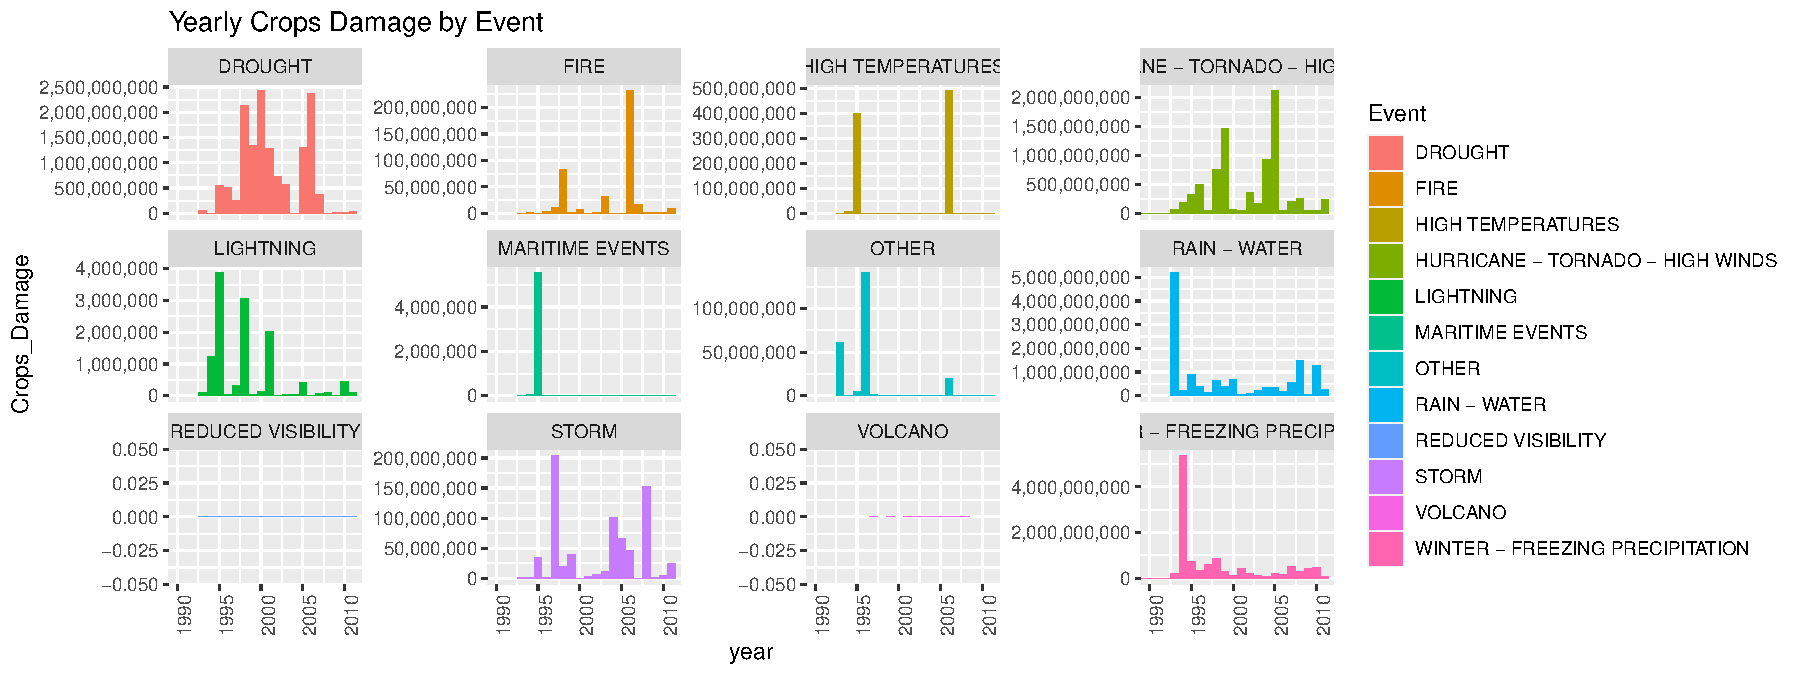
\includegraphics{RepData_PeerAssessment2_files/figure-latex/Crops Results-2.pdf}

In turn, (1) Droughts, (2) Heavy Rain and Floods and others, and (3)
Winter/Freezing events, in that same order, cause the most damage to
crops, which, upon further thinking, it's not really surprising.
Although different crops require different nurturing, for example, corn
requires relative little water, whereas bananas require a lot, not to
mention the temperature issue, these events escape the status quo
specific to each crop, EVEN if, over decades, if not hundreds of years,
their location/area has been planned for.

It is worth noticing that, the Rain Water category created for this
analysis only becomes ``relevant'' because of a VERY NOTICEABLE spike,
though this spike of damage said category causes to property and crops
take place in years very apart one from the other. So the questions is
raised again, is there a lack of data or its consistency? Still, even if
said spikes are noticeable, the property damage spike exceeds 112
billion USDs, whereas the spike in crops damage barely exceeds 5
billion.

So, did this event become harsher in said years, or is it a matter of
frequency? And could the same be contemplated for the other events?

\hypertarget{still-ultimately-droughts-are-the-most-damaging-for-crops-accumulated-over-the-years-and-even-consistently-across-time.}{%
\paragraph{Still, ultimately, Droughts are the most damaging for crops,
accumulated over the years and even consistently across
time.}\label{still-ultimately-droughts-are-the-most-damaging-for-crops-accumulated-over-the-years-and-even-consistently-across-time.}}

Though it's important to mention that, prior to 1990, there seem to be a
lack of observations for all events, even hurricanes, which is why the
timeframe prior to 1990 was cut off from the plots.

\begin{Shaded}
\begin{Highlighting}[]
\FunctionTok{library}\NormalTok{(ggplot2)}
\FunctionTok{options}\NormalTok{(}\AttributeTok{scipen=}\DecValTok{999}\NormalTok{)}

\NormalTok{injuries }\OtherTok{\textless{}{-}} \FunctionTok{ggplot}\NormalTok{(Casualties\_total, }\FunctionTok{aes}\NormalTok{(Event, Injuries))}
\NormalTok{injuries }\OtherTok{\textless{}{-}}\NormalTok{ injuries }\SpecialCharTok{+} \FunctionTok{geom\_bar}\NormalTok{(}\AttributeTok{stat=}\StringTok{"identity"}\NormalTok{, }\AttributeTok{position =} \StringTok{"dodge"}\NormalTok{) }\SpecialCharTok{+} \FunctionTok{ggtitle}\NormalTok{(}\StringTok{"Injuries vs Event Category"}\NormalTok{) }\SpecialCharTok{+} \FunctionTok{theme}\NormalTok{(}\AttributeTok{axis.text.x =} \FunctionTok{element\_text}\NormalTok{(}\AttributeTok{angle =} \DecValTok{90}\NormalTok{))}
\NormalTok{injuries }\OtherTok{\textless{}{-}}\NormalTok{ injuries }\SpecialCharTok{+} \FunctionTok{scale\_y\_continuous}\NormalTok{(}\AttributeTok{labels =}\NormalTok{ scales}\SpecialCharTok{::}\NormalTok{comma)}
\FunctionTok{print}\NormalTok{(injuries)}
\end{Highlighting}
\end{Shaded}

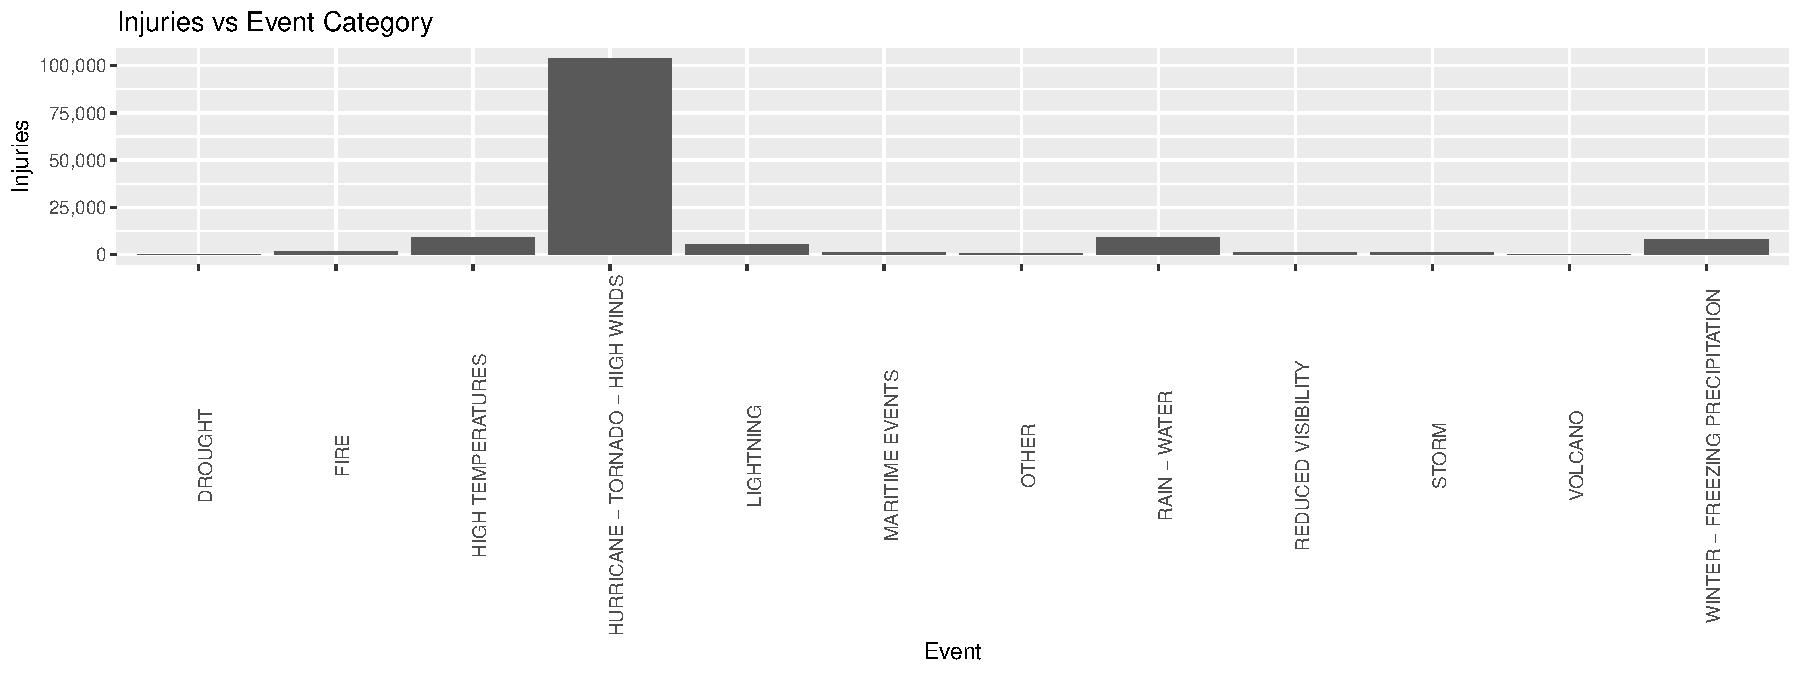
\includegraphics{RepData_PeerAssessment2_files/figure-latex/Injuries Results-1.pdf}

\begin{Shaded}
\begin{Highlighting}[]
\NormalTok{injuries\_vs\_year}\OtherTok{\textless{}{-}} \FunctionTok{ggplot}\NormalTok{(Casualties\_aggregation, }\FunctionTok{aes}\NormalTok{(year, Injuries, }\AttributeTok{fill =}\NormalTok{ Event))}
\NormalTok{injuries\_vs\_year }\OtherTok{\textless{}{-}}\NormalTok{ injuries\_vs\_year }\SpecialCharTok{+} \FunctionTok{geom\_bar}\NormalTok{(}\AttributeTok{stat=}\StringTok{"identity"}\NormalTok{, }\AttributeTok{position =} \StringTok{"dodge"}\NormalTok{) }\SpecialCharTok{+} \FunctionTok{ggtitle}\NormalTok{(}\StringTok{"Yearly Injuries by Event"}\NormalTok{)}\SpecialCharTok{+} \FunctionTok{facet\_wrap}\NormalTok{(.}\SpecialCharTok{\textasciitilde{}}\NormalTok{Event, }\AttributeTok{scales =} \StringTok{"free\_y"}\NormalTok{) }\SpecialCharTok{+} \FunctionTok{theme}\NormalTok{(}\AttributeTok{axis.text.x =} \FunctionTok{element\_text}\NormalTok{(}\AttributeTok{angle =} \DecValTok{90}\NormalTok{))}
\NormalTok{injuries\_vs\_year }\OtherTok{\textless{}{-}}\NormalTok{ injuries\_vs\_year  }\SpecialCharTok{+} \FunctionTok{scale\_y\_continuous}\NormalTok{(}\AttributeTok{labels =}\NormalTok{ scales}\SpecialCharTok{::}\NormalTok{comma)}
\FunctionTok{print}\NormalTok{(injuries\_vs\_year)}
\end{Highlighting}
\end{Shaded}

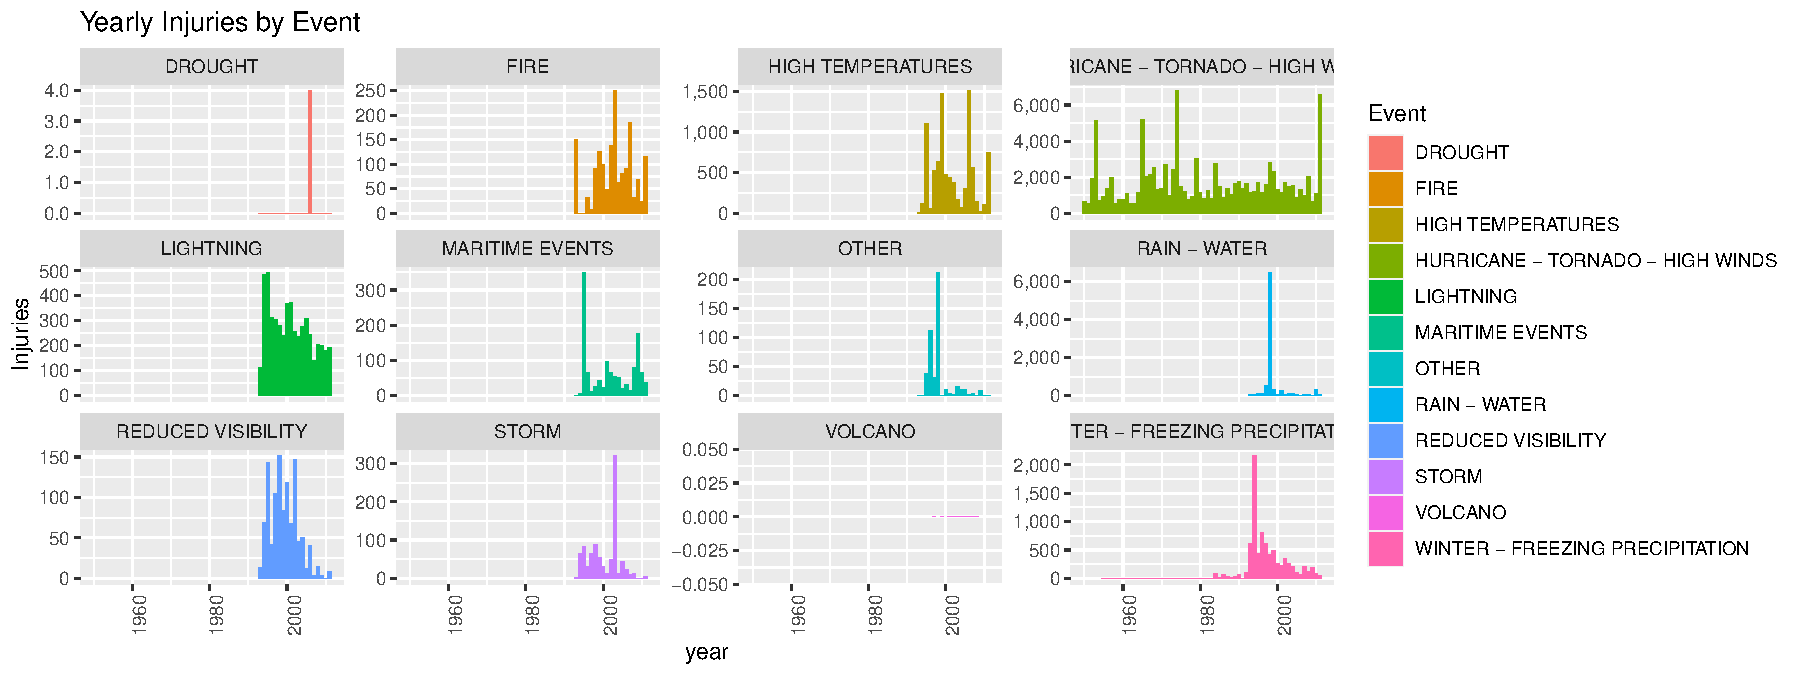
\includegraphics{RepData_PeerAssessment2_files/figure-latex/Injuries Results-2.pdf}

As for injuries, there is no question that consistently, during the
years, hundreds and even thousands can be attributed to Hurricanes and
Tornadoes, which in turn give said category the 1° place overall, or
accumulated over the years.

\hypertarget{hurricanes-tornadoes-and-high-winds-are-the-weather-events-that-leave-the-most-injured-in-their-wake-though-this-could-be-attributed-to-the-increasingly-evident-lack-of-data-prior-to-1990.}{%
\paragraph{Hurricanes, Tornadoes and High Winds are the weather events
that leave the most injured in their wake, though this could be
attributed to the increasingly evident lack of data prior to
1990.}\label{hurricanes-tornadoes-and-high-winds-are-the-weather-events-that-leave-the-most-injured-in-their-wake-though-this-could-be-attributed-to-the-increasingly-evident-lack-of-data-prior-to-1990.}}

\begin{Shaded}
\begin{Highlighting}[]
\FunctionTok{library}\NormalTok{(ggplot2)}
\FunctionTok{options}\NormalTok{(}\AttributeTok{scipen=}\DecValTok{999}\NormalTok{)}

\NormalTok{fatalities }\OtherTok{\textless{}{-}} \FunctionTok{ggplot}\NormalTok{(Casualties\_total, }\FunctionTok{aes}\NormalTok{(Event, Fatalities))}
\NormalTok{fatalities }\OtherTok{\textless{}{-}}\NormalTok{ fatalities }\SpecialCharTok{+} \FunctionTok{geom\_bar}\NormalTok{(}\AttributeTok{stat=}\StringTok{"identity"}\NormalTok{, }\AttributeTok{position =} \StringTok{"dodge"}\NormalTok{) }\SpecialCharTok{+} \FunctionTok{ggtitle}\NormalTok{(}\StringTok{"Fatalities vs Event Category"}\NormalTok{) }\SpecialCharTok{+} \FunctionTok{theme}\NormalTok{(}\AttributeTok{axis.text.x =} \FunctionTok{element\_text}\NormalTok{(}\AttributeTok{angle =} \DecValTok{90}\NormalTok{))}
\NormalTok{fatalities }\OtherTok{\textless{}{-}}\NormalTok{ fatalities }\SpecialCharTok{+} \FunctionTok{scale\_y\_continuous}\NormalTok{(}\AttributeTok{labels =}\NormalTok{ scales}\SpecialCharTok{::}\NormalTok{comma)}
\FunctionTok{print}\NormalTok{(fatalities)}
\end{Highlighting}
\end{Shaded}

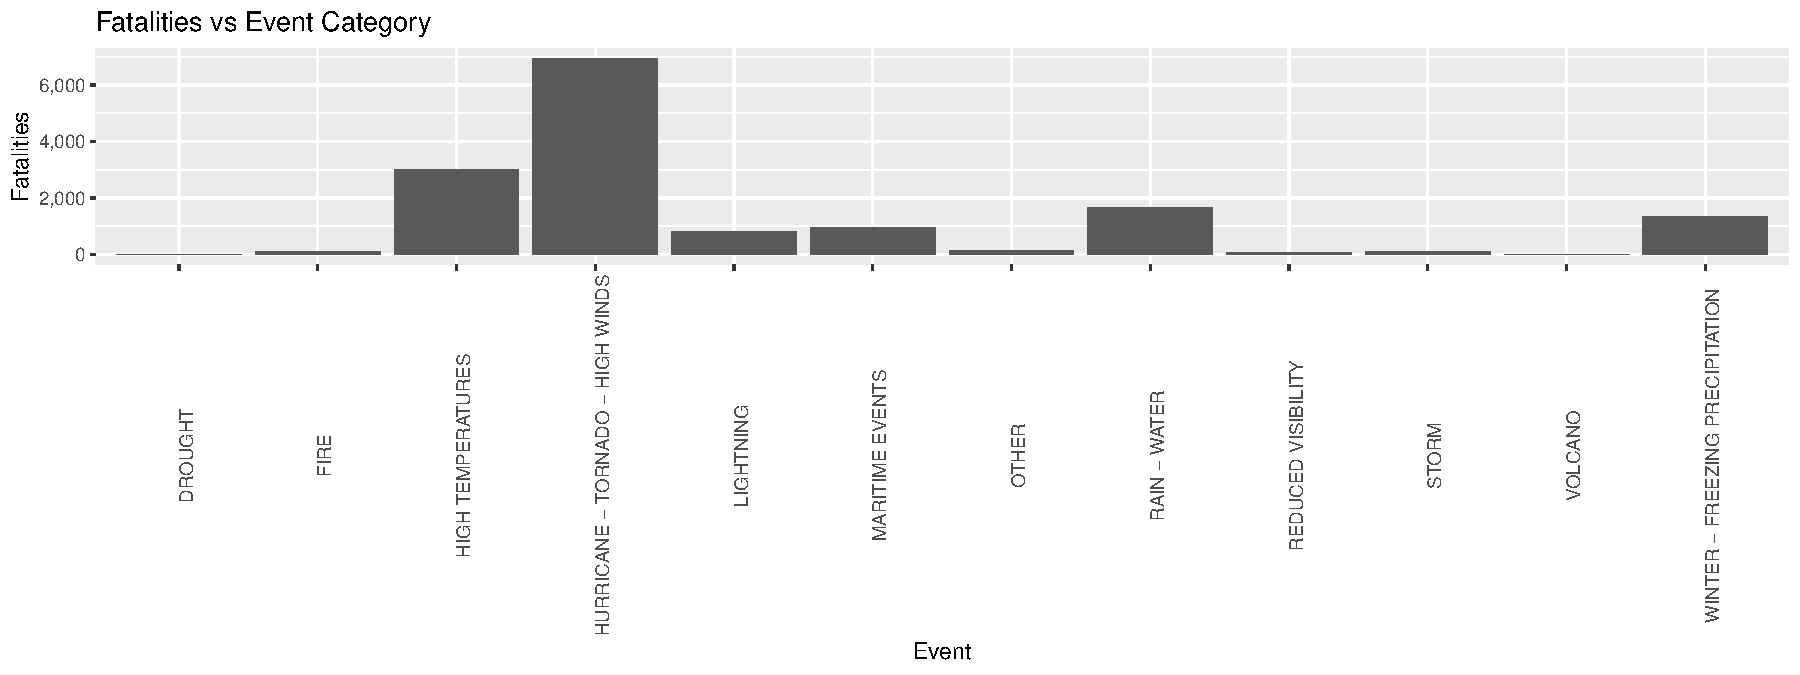
\includegraphics{RepData_PeerAssessment2_files/figure-latex/Fatalities Results-1.pdf}

\begin{Shaded}
\begin{Highlighting}[]
\NormalTok{fatalities\_vs\_year}\OtherTok{\textless{}{-}} \FunctionTok{ggplot}\NormalTok{(Casualties\_aggregation, }\FunctionTok{aes}\NormalTok{(year, Fatalities, }\AttributeTok{fill =}\NormalTok{ Event))}
\NormalTok{fatalities\_vs\_year }\OtherTok{\textless{}{-}}\NormalTok{ fatalities\_vs\_year }\SpecialCharTok{+} \FunctionTok{geom\_bar}\NormalTok{(}\AttributeTok{stat=}\StringTok{"identity"}\NormalTok{, }\AttributeTok{position =} \StringTok{"dodge"}\NormalTok{) }\SpecialCharTok{+} \FunctionTok{ggtitle}\NormalTok{(}\StringTok{"Yearly Fatalities by Event"}\NormalTok{)}\SpecialCharTok{+} \FunctionTok{facet\_wrap}\NormalTok{(.}\SpecialCharTok{\textasciitilde{}}\NormalTok{Event, }\AttributeTok{scales =} \StringTok{"free\_y"}\NormalTok{) }\SpecialCharTok{+} \FunctionTok{theme}\NormalTok{(}\AttributeTok{axis.text.x =} \FunctionTok{element\_text}\NormalTok{(}\AttributeTok{angle =} \DecValTok{90}\NormalTok{))}
\NormalTok{fatalities\_vs\_year }\OtherTok{\textless{}{-}}\NormalTok{ fatalities\_vs\_year  }\SpecialCharTok{+} \FunctionTok{scale\_y\_continuous}\NormalTok{(}\AttributeTok{labels =}\NormalTok{ scales}\SpecialCharTok{::}\NormalTok{comma)}
\FunctionTok{print}\NormalTok{(fatalities\_vs\_year)}
\end{Highlighting}
\end{Shaded}

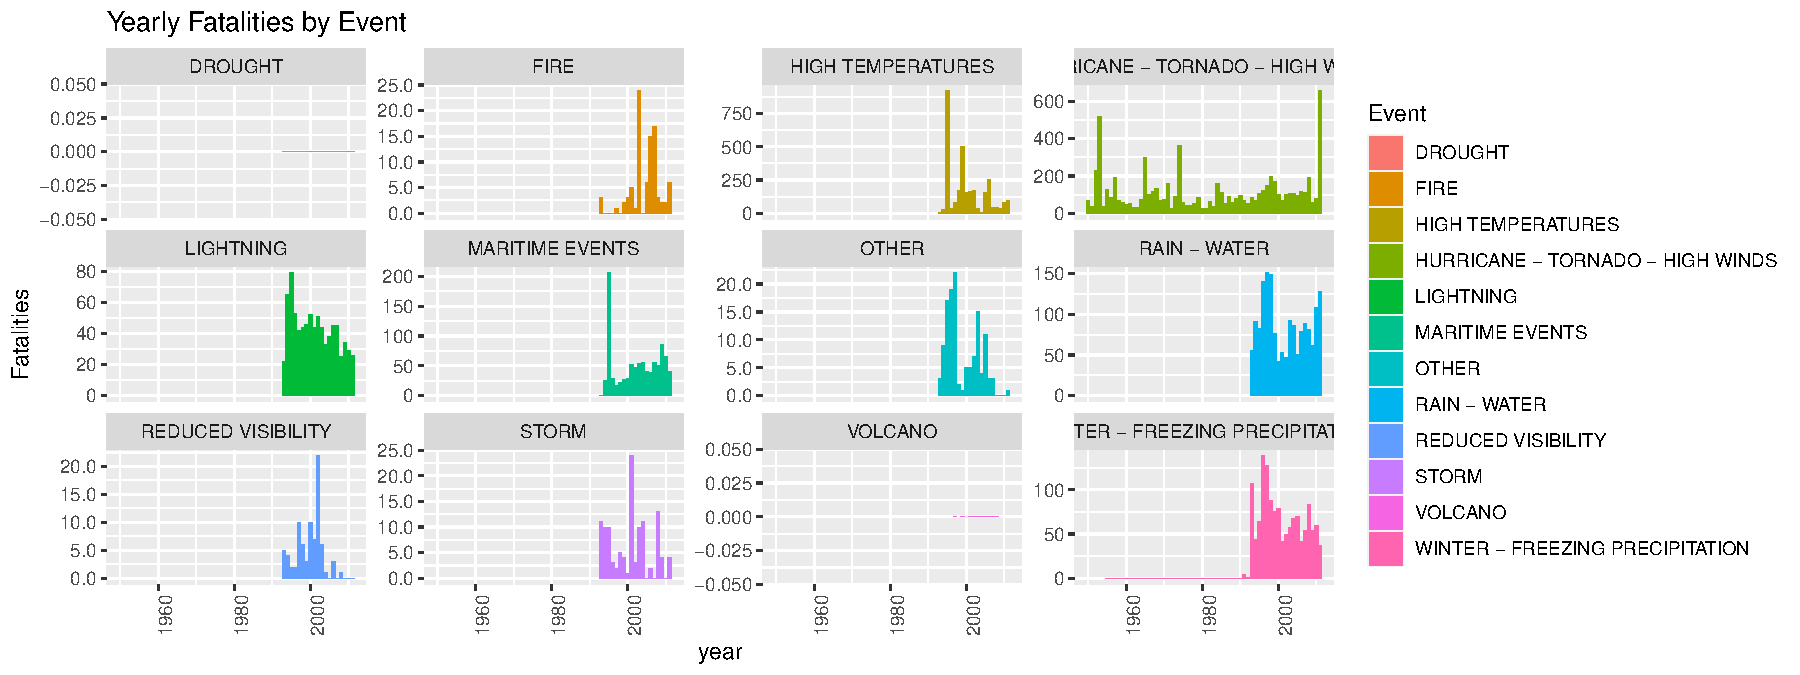
\includegraphics{RepData_PeerAssessment2_files/figure-latex/Fatalities Results-2.pdf}

\begin{Shaded}
\begin{Highlighting}[]
\FunctionTok{rm}\NormalTok{(}\AttributeTok{list=}\FunctionTok{ls}\NormalTok{())}
\end{Highlighting}
\end{Shaded}

Finally, Hurricanes, Tornadoes and High Winds are the events that cause
the most deaths among weather events. HOWEVER, this event's deaths are
measured since 1940, whereas other events since after 1990. In that
regard, most deaths by hurricane amount to less than 200, and likely
half the time, they even amount to no more than 50-something.

On the other hand, Rain and Water events, Winter and Freezing events,
High Temperatures events, Maritime Events, and even Lightnings, are
comparatively as deadly, if not more, than Hurricanes, when the spikes
are ignored, and if all were measured since 1990.

\hypertarget{so-hurricanes-tornadoes-and-high-winds-seem-to-be-the-most-deadly-probably-because-of-some-clear-spikes-and-likely-due-to-a-lack-of-data-prior-to-1990-for-the-other-events.}{%
\paragraph{So, Hurricanes, Tornadoes and High Winds seem to be the most
deadly, probably because of some clear spikes, and likely due to a lack
of data prior to 1990 for the other
events.}\label{so-hurricanes-tornadoes-and-high-winds-seem-to-be-the-most-deadly-probably-because-of-some-clear-spikes-and-likely-due-to-a-lack-of-data-prior-to-1990-for-the-other-events.}}

\hypertarget{conclusions-and-closing-words}{%
\subsection{Conclusions and Closing
Words}\label{conclusions-and-closing-words}}

The AVAILABLE data (though the transformation of factors K, B, M, etc.
might be part of the cause) shows that:

\begin{itemize}
\item
  Hurricanes, Tornadoes, Rain and Floods are the most damaging for
  property.
\item
  Droughts, Heavy Rain and Floods, and Winter-Freezing precipitation are
  the most damaging for crops.
\item
  Hurricanes and Tornadoes leave the most injured in their wake,
  consistently across time and accumulated between 1960 and 2011.
\item
  Hurricanes and Tornadoes ALSO leave the most dead in their wake.
\end{itemize}

However, the database seems to be lacking, as it makes no sense that
only hurricanes, tornadoes and the like have caused damage, injuries and
death prior to 1990.

Still, attempting to determine the most damaging and/or deadly event by
aggregating the data is too simplistic. And though adding the time
variable might offer a more comprehensive view in the issue, it is not
enough.

In order to properly answer these questions, a risk management approach
is necessary, and one would have to:

\begin{enumerate}
\def\labelenumi{(\arabic{enumi})}
\item
  Estimate the probability that, any given day, one of the events can
  take place, for each year, by simply measuring the relative frequency.
\item
  Aggregate the damage/injured/dead by year and event, and multiply that
  value by the probability estimated by event and year.
\item
  Ignore all observations prior to 1980 or 1990.
\end{enumerate}

In that way, the accumulated damage and yearly damage can be compared,
all relative to the likeness the events took place, all within the same
timeframe.

\end{document}
